% !TeX spellcheck = fr_CA
\documentclass[letterpaper, 12pt]{article}

% Encoding
\usepackage[utf8]{inputenc}
\usepackage[T1]{fontenc}

% Margins
\usepackage[top=2.5cm, bottom=2.5cm, left=2.5cm, right=2.5cm]{geometry}
% One half spacing
\usepackage{setspace}
\onehalfspacing
% Paragraph indentation
\setlength{\parindent}{0cm}
% Page numbering to the right
\usepackage{fancyhdr}
\pagestyle{fancy}
\fancypagestyle{plain}{\pagestyle{fancy}}
\fancyhf{} % clear all header and footer fields
\fancyfoot[R]{\thepage}
\renewcommand{\headrulewidth}{0cm}
\renewcommand{\footrulewidth}{0cm}
% Footnotes
\usepackage[bottom]{footmisc}

% Abstract
\usepackage{abstract}
% Table of contents, list of figures and tables
\usepackage{tocloft}
\usepackage[notindex, nottoc, notlof, notlot]{tocbibind}
% List of abbreviations
\usepackage{nomencl}
\makenomenclature
% Appendices
\usepackage[title, titletoc]{appendix}
% Bibliography
\usepackage[numbers]{natbib}
\usepackage{url}
\def\UrlBreaks{\do\/\do-}

% Figures
\usepackage{float, graphicx}
% Tables
\usepackage{booktabs, longtable, fonttable}
% SI units
\usepackage[squaren, Gray]{SIunits}
% Mathematics
\usepackage{amsmath, amssymb, mathrsfs}
% Drawings
\usepackage{tikz}
% Hypertext
\usepackage[colorlinks=false, pdfborder={0 0 0}]{hyperref}

% Document in french
\usepackage[french]{babel}

\usepackage{listings}
\usepackage{pdflscape}

% Matrice augmenté
\makeatletter
\renewcommand*\env@matrix[1][*\c@MaxMatrixCols c]{%
    \hskip -\arraycolsep
    \let\@ifnextchar\new@ifnextchar
    \array{#1}}
\makeatother

\newcommand{\matr}[1]{\mathbf{#1}}

\begin{document}
    % Title page
    \begin{titlepage}
        \begin{center}
            \begin{large}
                \textbf{FACULTÉ DES SCIENCES} \\
                \textbf{DÉPARTEMENT D'INFORMATIQUE}
            \end{large}
            \vfill
            \begin{Large}
                \textbf{IFT725 - Réseaux neuronaux} \\
                Projet - \textit{Curious Network}
            \end{Large}
            \vfill
            \textit{préparé par} \\
            \begin{tabular}{ccc}
                \textbf{Gabriel Gibeau Sanchez (gibg2501)} \\
                \textbf{Marc-Antoine Maheux (mahm1904)} \\
                \textbf{Aurélien Vauthier (vaua2803)}
            \end{tabular}
            \vfill
            \textit{présenté à} \\
            \textbf{Pierre-Marc Jodoin} \\
            \vfill
            11 avril 2020
        \end{center}
    \end{titlepage}
    \pagebreak
    
    \pagenumbering{roman}
    
    % Table of contents
    \tableofcontents
    \pagebreak
    
    % List of figures
    %\renewcommand{\listfigurename}{Liste des figures}
    \renewcommand{\figurename}{Figure}
    \renewcommand{\cftfigpresnum}{Figure }
    \renewcommand{\cftfignumwidth}{2cm}
    \listoffigures
    \pagebreak
%    
%    % List of tables
    \renewcommand{\tablename}{Tableau}
    \renewcommand{\cfttabpresnum}{Tableau }
    \renewcommand{\cfttabnumwidth}{2cm}
    \listoftables
    \pagebreak
    
    % List of abbreviations
    %\renewcommand{\nomname}{Liste des symboles et abréviations}
    %\renewcommand{\nomlabel}[1]{\hfil #1 \hfil}
    %\printnomenclature
    %\pagebreak
    
    \pagenumbering{arabic}
    \section{Mise en contexte}
    Dans un contexte de robotique, la puissance de calcul et la mémoire sont limitées, il faut donc optimiser l'utilisation des ressources au maximum. Malheureusement, il est nécessaire d’avoir une vaste quantité de stimuli provenant de différents capteurs (caméra RGB, caméra 3D, LIDAR, matrice de microphones, ...) pour rendre un robot le plus autonome possible. Ainsi, il y a trop de stimuli pour faire un traitement détaillé de chacun de ceux-ci avec les ressources embarquées. Puisqu’il est fort probable que seulement un sous-ensemble des stimuli soit important à un moment donné, il n’est donc pas nécessaire de tous les traiter simultanément. Il est intéressant de jeter un coup d'oeil à l'humain pour savoir comment il arrive à gérer tous les stimuli. L’être humain possède un mécanisme d’attention sélective permettant de se concentrer sur les stimuli les plus utiles au moment présent.
    \bigskip
    
    L’architecture robotique HBBA (\textit{Hybrid Behavior-Based Architecture})  [1, 2, 3] possède un mécanisme d’attention sélective fonctionnant à l’aide de filtres à décimation. Par exemple, un filtre à décimation sur un signal vidéo permet de traiter une image sur \(N\), où \(N\) est un paramètre du filtre. Ce mécanisme d’attention sélective permet de réduire les ressources utilisées sur un robot pour permettre l’exécution d’autres traitements qu’il serait impossible de réaliser sans ce mécanisme. Dans l’architecture robotique HBBA, les filtres à décimation sont paramétrés par le développeur à l'aide de désirs et de stratégies. Il serait intéressant que le robot fasse cette paramétrisation de façon autonome. Un signal de curiosité serait en mesure de faire cela. Plus un stimulus possède un signal de curiosité élevé, plus le paramètre \(N\) de ce filtre doit être faible. Il est possible de  générer un signal de curiosité à l’aide d’un auto-encodeur. L’erreur de reconstruction d’un auto-encodeur peut être utilisée comme signal de curiosité. Si l'erreur de reconstruction est élevée pour un stimulus, alors le robot n'a jamais rencontré cette situation pour le sens (le capteur) d’où provient ce stimulus, donc le robot devrait être curieux pour ce sens. Pour que le robot soit en mesure ne pas donner son attention toujours au même stimulus, le signal de curiosité doit diminuer à force que le même stimulus est senti.
    \bigskip
    
    Pour utiliser un signal de curiosité pour la paramétrisation des filtres à décimation, il est important que la génération des signaux de curiosité n’utilise que peu de ressources. Il est possible d’utiliser des auto-encodeurs utilisant les données brutes des capteurs, mais ceci a le potentiel d’utiliser trop de ressources. La question suivante se pose : est-il possible d’utiliser des caractéristiques décrivant les stimuli au lieu des données brutes? La réponse est oui. Un réseau de neurones pourrait extraire des caractéristiques que l’auto-encodeur pourrait utiliser pour générer le signal de curiosité. Cette architecture de réseaux de neurones a été utilisée dans un contexte d’exploration d’un environnement à l’aide d’apprentissage par renforcement et d’un signal de curiosité [4]. L’utilisation de caractéristiques au lieu des pixels leur a permis d’améliorer les performances. Pour assurer la diminution du signal de curiosité dans le temps, l’entraînement des réseaux de neurones doit se faire en ligne. L’apprentissage se fait de manière non supervisée en diminuant les signaux de curiosité (erreurs de reconstruction).

\section{Définition du projet}
    \label{sec:definition_projet}
    Afin de respecter le temps qu’il est possible d’accorder au projet, le générateur de signaux de curiosité sera implémenté pour un cas d’utilisation simplifié. Les stimuli seront des images RGB provenant d’une caméra filmant en  Full HD (1920x1080). Les images Full HD seront divisées en 144 régions de 120x120 pixels qui seront considérés comme des images provenant de caméras différentes. Les images de ces régions seront des stimuli à part entière. Pour simplifier le projet, une région peut avoir l’attention ou non (\(N = \infty\)). Aucune attention partielle ne sera considérée. L’objectif est donc d’indiquer au robot une zone approximative de l’image Full HD où il doit focaliser son attention. Dans le cas non simplifié, l’objectif serait de changer le paramètre \(N\) de chacun des filtres à décimation de chaque stimulus en fonction de la valeur du signal de curiosité pour ce stimulus (chaque capteur génère un seul stimulus).
    
    Par exemple, si notre modèle est entraîné sur des images de murs sans affiche, alors une affiche sur un mur générerait des signaux de curiosité élevés pour les régions contenant l’affiche. L’attention sera donnée aux régions ayant un signal de curiosité supérieur à un certain seuil. Par conséquent, les régions correspondantes à l’affiche devraient avoir l’attention afin que le robot puisse traiter ces stimuli (par exemple, pour s’orienter vers l’affiche ou pour analyser le texte sur l’affiche). La figure \ref{fig:definition_sortie_reseau} présente l’exemple énoncé. 
    
    \pagebreak
    \begin{figure}[H]
        \centering
        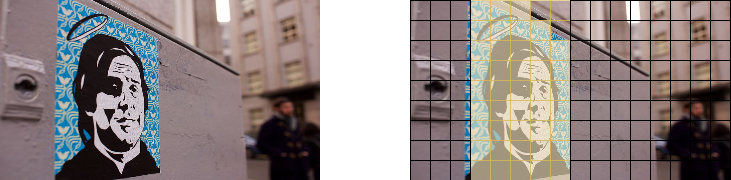
\includegraphics[width=15cm]{images/definition.png}
        \caption[Définition de la sortie du réseau]{Définition de la sortie du réseau\footnotemark}
        \label{fig:definition_sortie_reseau}
    \end{figure}
    \footnotetext{\url{https://www.peakpx.com/431428/pop-art-painting-on-white-wall}}
    \section{Création de la base de données}
    Afin d'entraîner les réseaux de neurones, deux bases de données ont été générées à partir de segments vidéo Full HD prises dans différents couloirs de l’Université de Sherbrooke: des couloirs où les murs sont vierges de toutes affiches, images ou autres fresques, et des couloirs où on retrouve des éléments hétéroclites qui devraient susciter la curiosité du robot lorsqu’il les verra pour la première fois.\\
    
    La première base de données a été créée à partir de segments vidéo des tunnels de l'Université de Sherbrooke. Le contenu des images pour l'entraînement correspond aux sections des tunnels n'ayant pas de fresque, tandis que le contenu des images de validation et de test correspond aux sections des tunnels ayant des fresques sur les murs. Cette base de données sera nommée par le terme base de données tunnel dans la suite du document. À l'aide de segments vidéo des quatrième et cinquième étages de la faculté de génie de l'Université de Sherbrooke, il a été possible de créer la deuxième base de données. Les images du quatrième étage sont utilisées pour l'entraînement, car il y a moins d'éléments sur les murs, tandis que les images du cinquième étage sont utilisées pour la validation et les tests parce qu'il y a plus d'éléments sur les murs. La deuxième base de données est jugée plus difficile, car il y a beaucoup de différence entre les images d'entraînement et celles de validation et de test. De plus, la complexité de l'environnement est plus grande. Cette base de données sera nommée par le terme base de données faculté de génie dans la suite du document.\\
    
    À fin de pouvoir comparer les différents réseaux développer à l'aide de métriques, il a été nécessaire de développer un outil permettant d'annoter les images de validation et de test. La figure \ref{fig:outil_annotation} présente l'interface d'annotation et la figure \ref{fig:outil_lecture} présente celle de lecture. Le code de ces deux interfaces graphiques se trouve dans le dossier \texttt{git/tools/labeling}. La méthode d'annotation se résume à indiquer les régions de l'image qui sont différentes des images d'entraînement. Dans les deux interfaces, les régions jugées comme différentes sont indiquées par des carrés rouges. Ceci était fait pour chacune des images de validation et de test. Puisque la méthode de détermination des régions différentes est plutôt subjective, il est fort probable qu'il y ait plusieurs erreurs d'annotation.
    
    \begin{figure}
        \centering
        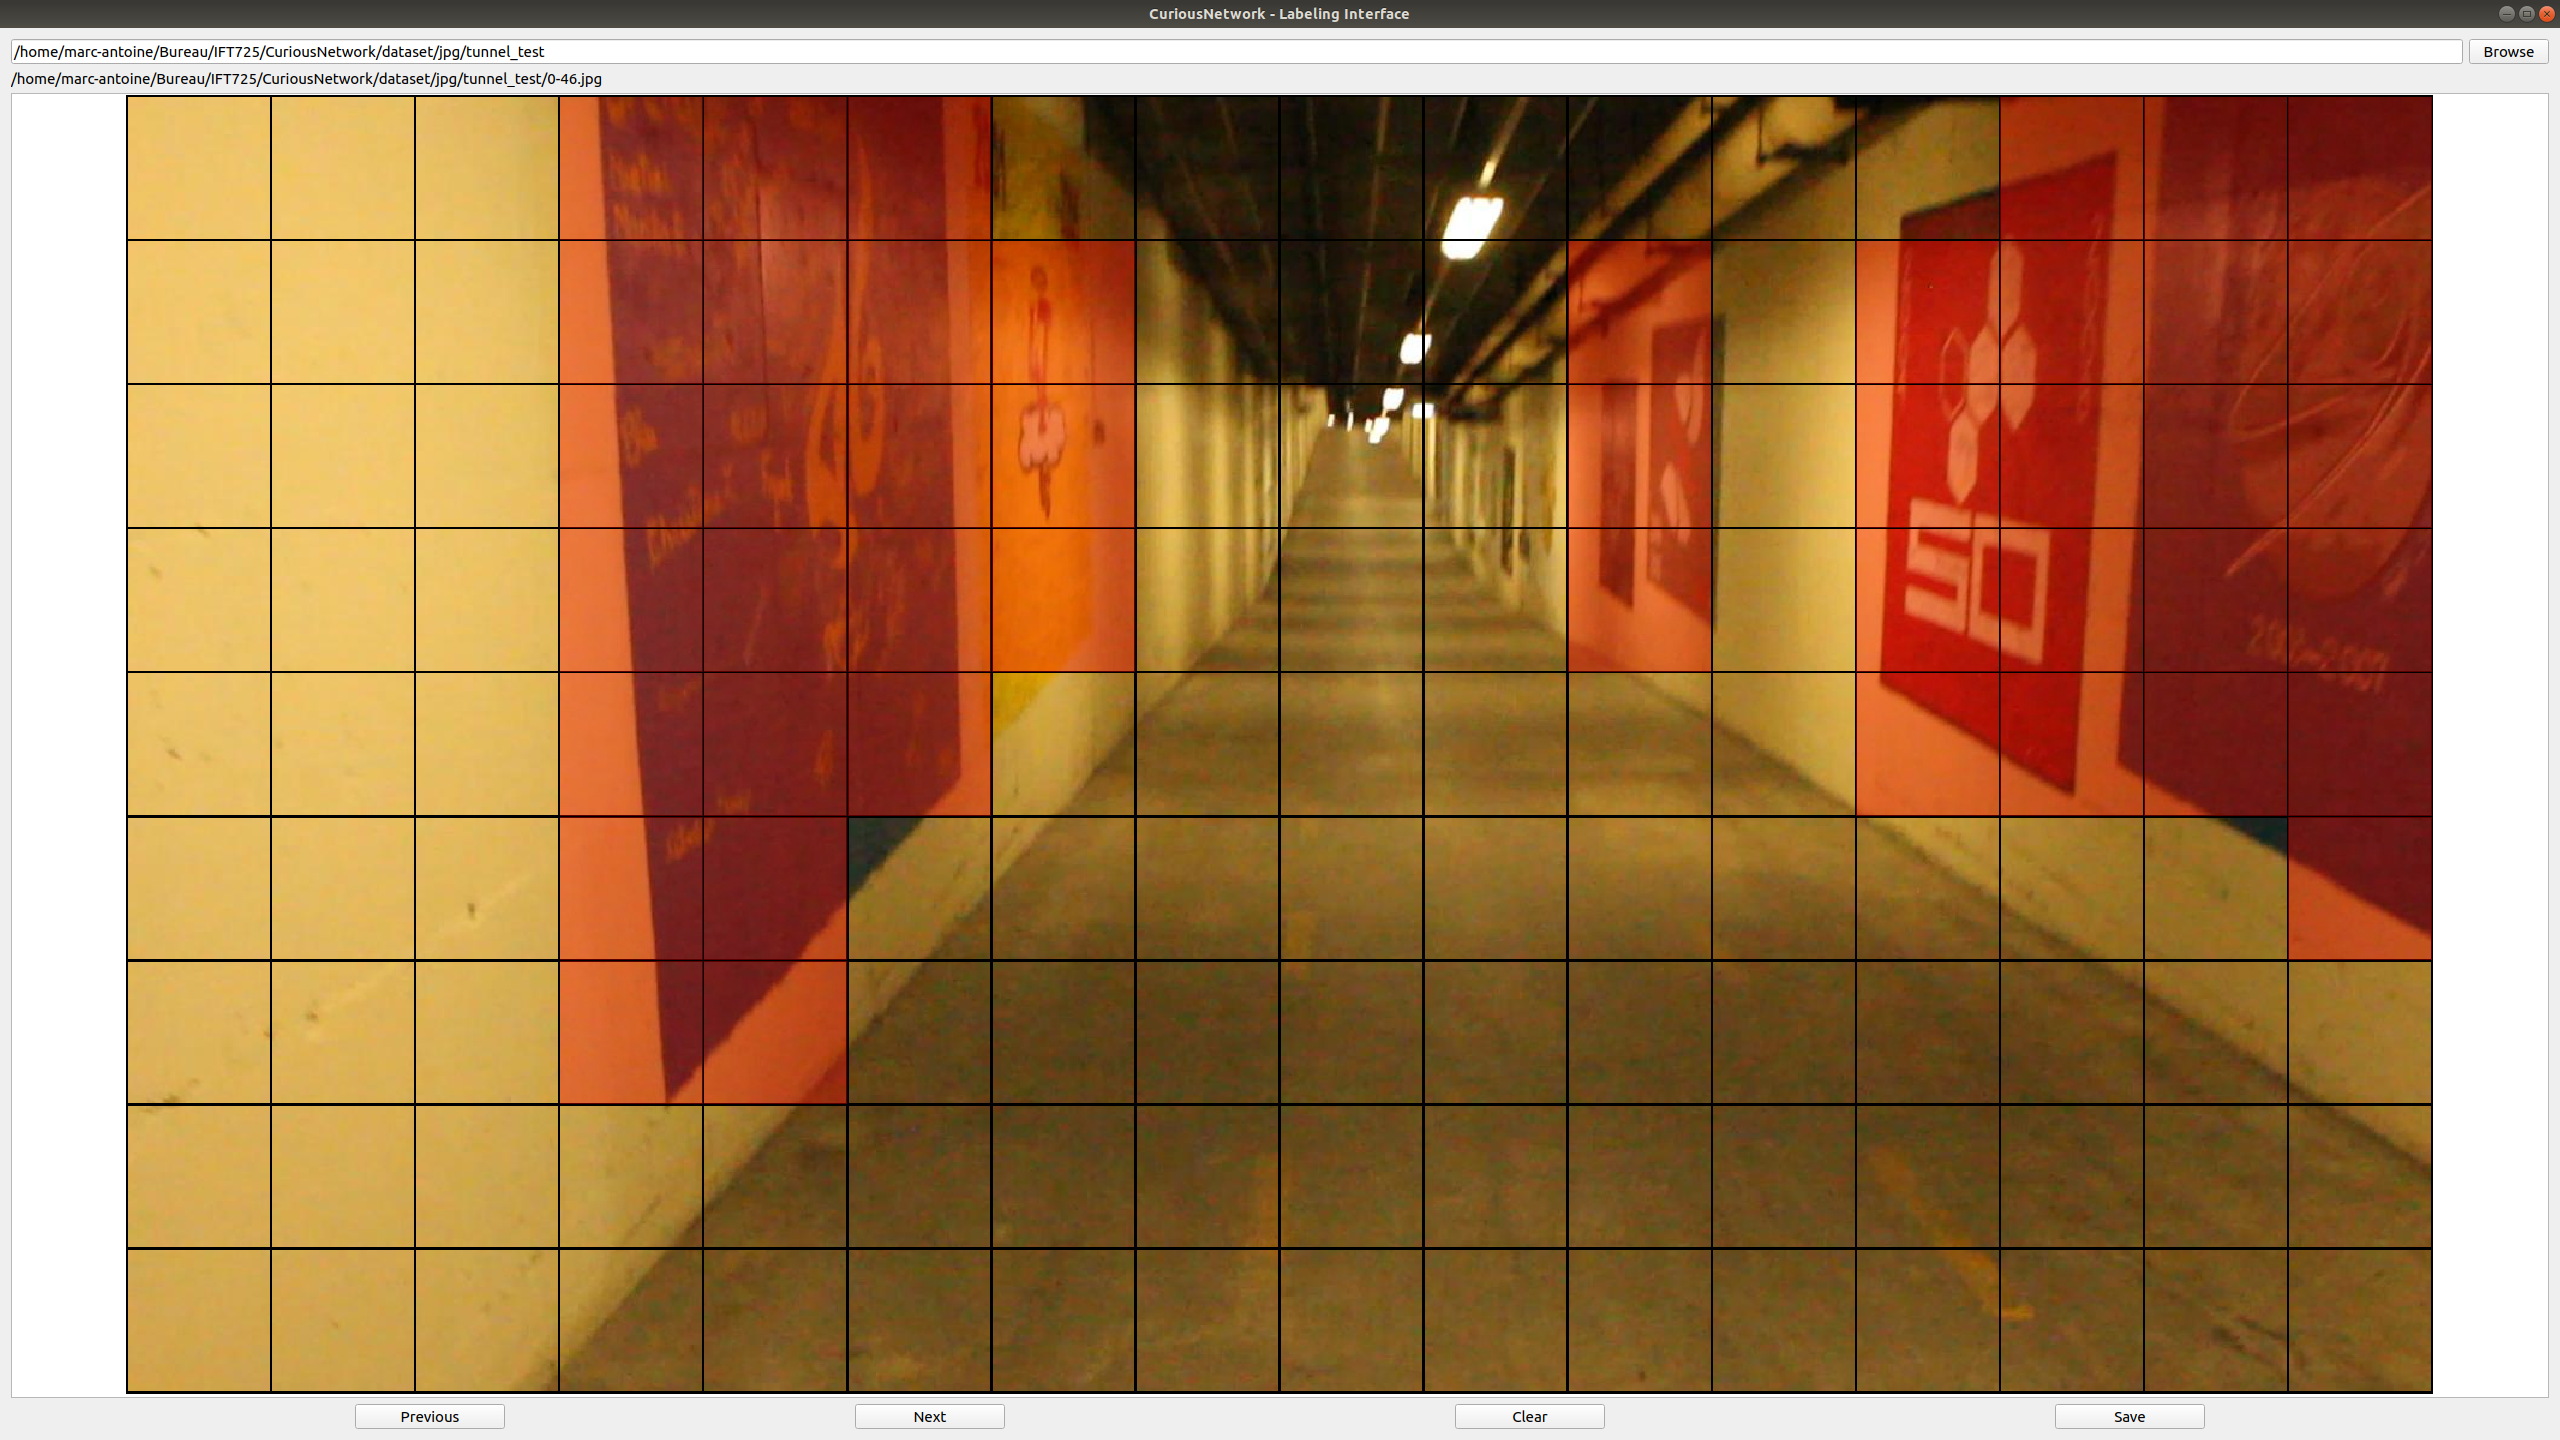
\includegraphics[width=15cm]{images/outil_annotation.png}
        \caption{Outil d'annotation des images}
        \label{fig:outil_annotation}
    \end{figure}

    \begin{figure}
        \centering
        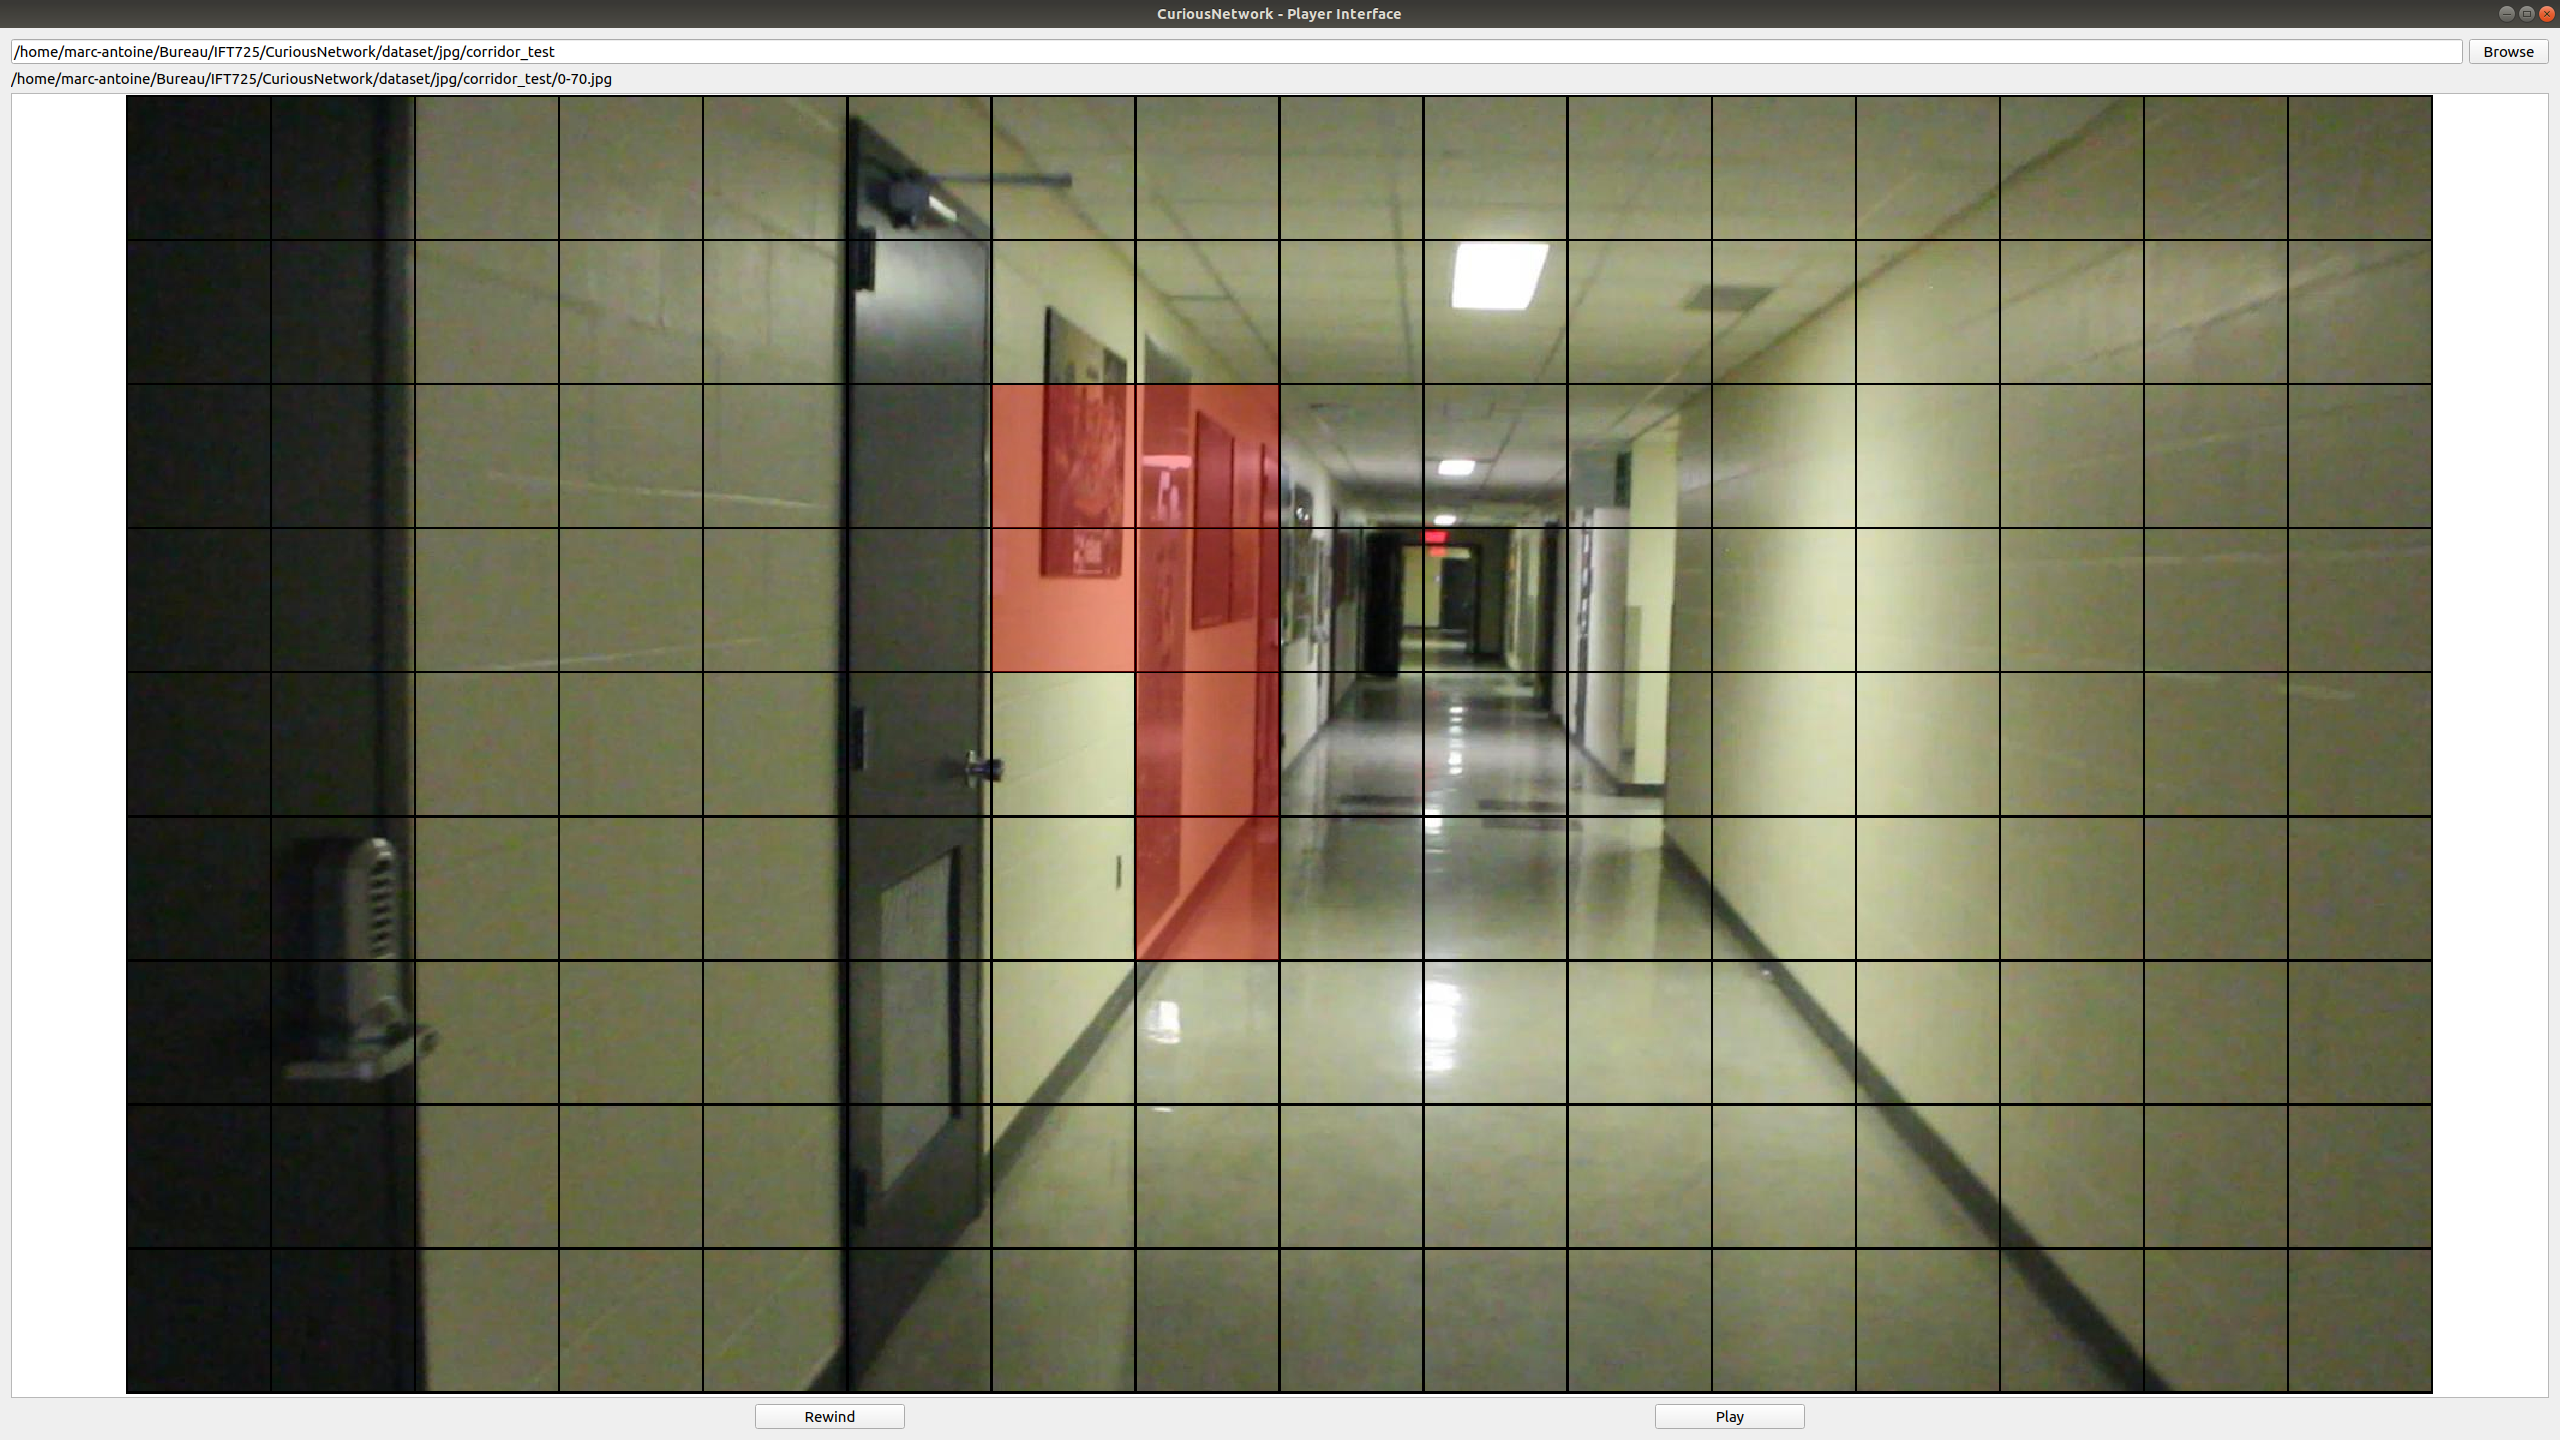
\includegraphics[width=15cm]{images/outil_lecture.png}
        \caption{Outil de lecture des images avec l'annotation}
        \label{fig:outil_lecture}
    \end{figure}

    Le tableau \ref{tab:nb_image_bd} présente le nombre d'images d'entraînement, de validation et de test pour chaque base de données. Puisque l'annotation des images est une tâche longue et fastidieuse et qu'elle ne fait pas partie du cadre du cours, il a été décidé d'annoter environ 1 000 images par base de données. Ce nombre a été jugé comme suffisant pour avoir une bonne idée de la performance des réseaux sans toutefois rendre la tâche d'annotation trop longue. Il a été préféré d'avoir plus d'images en test qu'en validation pour nous permettre d'avoir de bonnes métriques de test. De plus, les images de validation et de test sont semblables, mais n'ont pas le même contenu dans le but de ne pas fausser nos résultats de tests suite à un surentraînement des hyperparamètres sur les images de validation. 
    
    \begin{table}
        \centering
        \caption{Nombre d'images pour chaque base de données}
        \label{tab:nb_image_bd}
        \begin{tabular}{p{4cm}p{3cm}p{2.25cm}p{2.25cm}}
            \midrule
            Base de données &  Nombre d'images d'entraînement & Nombre d'images de validation & Nombre d'images de test\\
            \midrule\midrule
            Tunnel & 24 526 & 300 & 815\\
            Faculté de génie & 21 079 & 200 & 691\\
            \midrule
        \end{tabular}
    \end{table}

    \section{Conception}
    Dans le but de limiter l'utilisation de la mémoire et de réduire le temps d'entraînement, les réseaux de neurones n'utilisent pas les images Full HD (1920x1080) à l'entrée, mais plutôt des images redimensionnées par un facteur de 4. Les images d'entrée des réseaux de neurones ont une résolution de 480x270. La sortie de tous les réseaux de neurones correspond à une matrice d'erreur de 16x9 éléments parce que les images sont divisées en 144 régions comme décrit à la section \ref{sec:definition_projet}. Les régions ont une résolution 30x30 pour les images d'entrée des réseaux de neurones (120x120 pour les images Full HD). Pour l'ensemble des réseaux de neurones développés, le champ récepteur des neurones de sortie est de 60x60 (240x240 pour les images Full HD) parce que nous avons émis l'hypothèse que le voisinage de chaque région a une influence sur la région correspondant au neurone de sortie. Chaque élément de la matrice d'erreur de 16x9 correspond à l'erreur quadratique de reconstruction de la région de l'image d'entrée correspondante.\\
    
    Plusieurs réseaux de neurones ont été conçus pour déterminer le meilleur type de réseau à utiliser dans ce contexte. Certains sont des auto-encodeurs travaillant sur les pixels directement et d'autres ont un réseau de neurones pour l'extraction de caractéristiques, suivi d'un auto-encodeur travaillant sur les caractéristiques extraites. 

\subsection{Choix des métriques}
    L'entraînement se fait de façon non supervisée, donc il  a été décidé d'utiliser la fonction de coût d'entraînement du réseau définie par l'équation suivante. À l'aide de celle-ci, les réseaux de neurones apprennent à reconstruire les régions des images d'entraînement.
    
    \begin{equation}
        L = \sum_{i,j} \mathbf{S}_{i,j} \text{, où } \mathbf{S} \text{ est la matrice de sortie du réseau de neurone}
    \end{equation}
    
    Pour mesurer les performances des réseaux de neurones sur les données de validation et de test, l'utilisation des courbes ROC a été choisi puisque notre problème équivaut à un problème de classification deux classes où la classe est déterminée à l'aide d'un seuil. La courbe ROC est une bonne métrique dans ce cas. Pour permettre la comparaison des réseaux de neurones avec différents hyperparamètres et établir le meilleur type de réseau de neurones pour la situation, l'aire sous la courbe ROC a été utilisée. Plus l'aire sous la courbe est grande, plus que le réseau est bon. Pour calculer la courbe ROC, le nombre de vrais positifs et de faux positifs a été calculé pour différentes valeurs de seuil.

\subsection{Architecture des modèles}
    La figure \ref{fig:architecture_bloc_dense} présente l'architecture d'un bloc dense utilisé dans certains réseaux de neurones. Ce bloc peut être configuré à l'aide de \(N_C\) et de \(t\). 
    \begin{figure}[H]
        \centering
        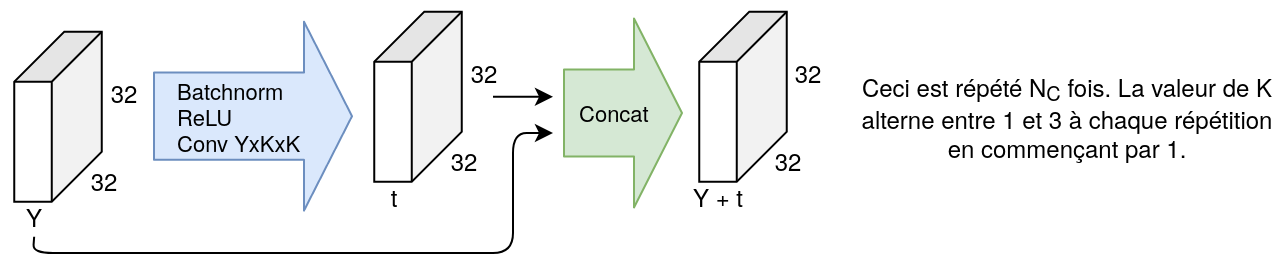
\includegraphics[width=12cm]{images/Architecture_DenseBlock.png}
        \caption{Architecture d'un bloc dense}
        \label{fig:architecture_bloc_dense}
    \end{figure}

    Certains réseaux de neurones font l'extraction de caractéristiques pour ensuite les utiliser dans un auto-encodeur. Tous ces réseaux utilisent le même auto-encodeur. Son architecture est présentée à la figure  \ref{fig:architecture_autoencoder_caracteristique}. L'entrée possède un nombre variable de canaux en entrée et a la même taille que la matrice d'erreurs. Ceci est dans le but que chaque vecteur de dimensions \(N_C\)x1x1 du tenseur d'entrée de dimensions \(N_C\)x16x9 correspond aux caractéristiques de chaque région de l'image. Les couches de ce réseau de neurones sont composées de convolutions 1x1 et de ReLU. Le nombre de canaux diminue à chaque couche dans l'encodeur et augmente dans le décodeur. Par conséquent, l'auto-encodeur apprend à réduire la dimensionnalité des caractéristiques de chaque région de l'image. La sortie de l'auto-encodeur correspond à l'erreur de reconstruction des caractéristiques des régions.
    \begin{figure}[H]
        \centering
        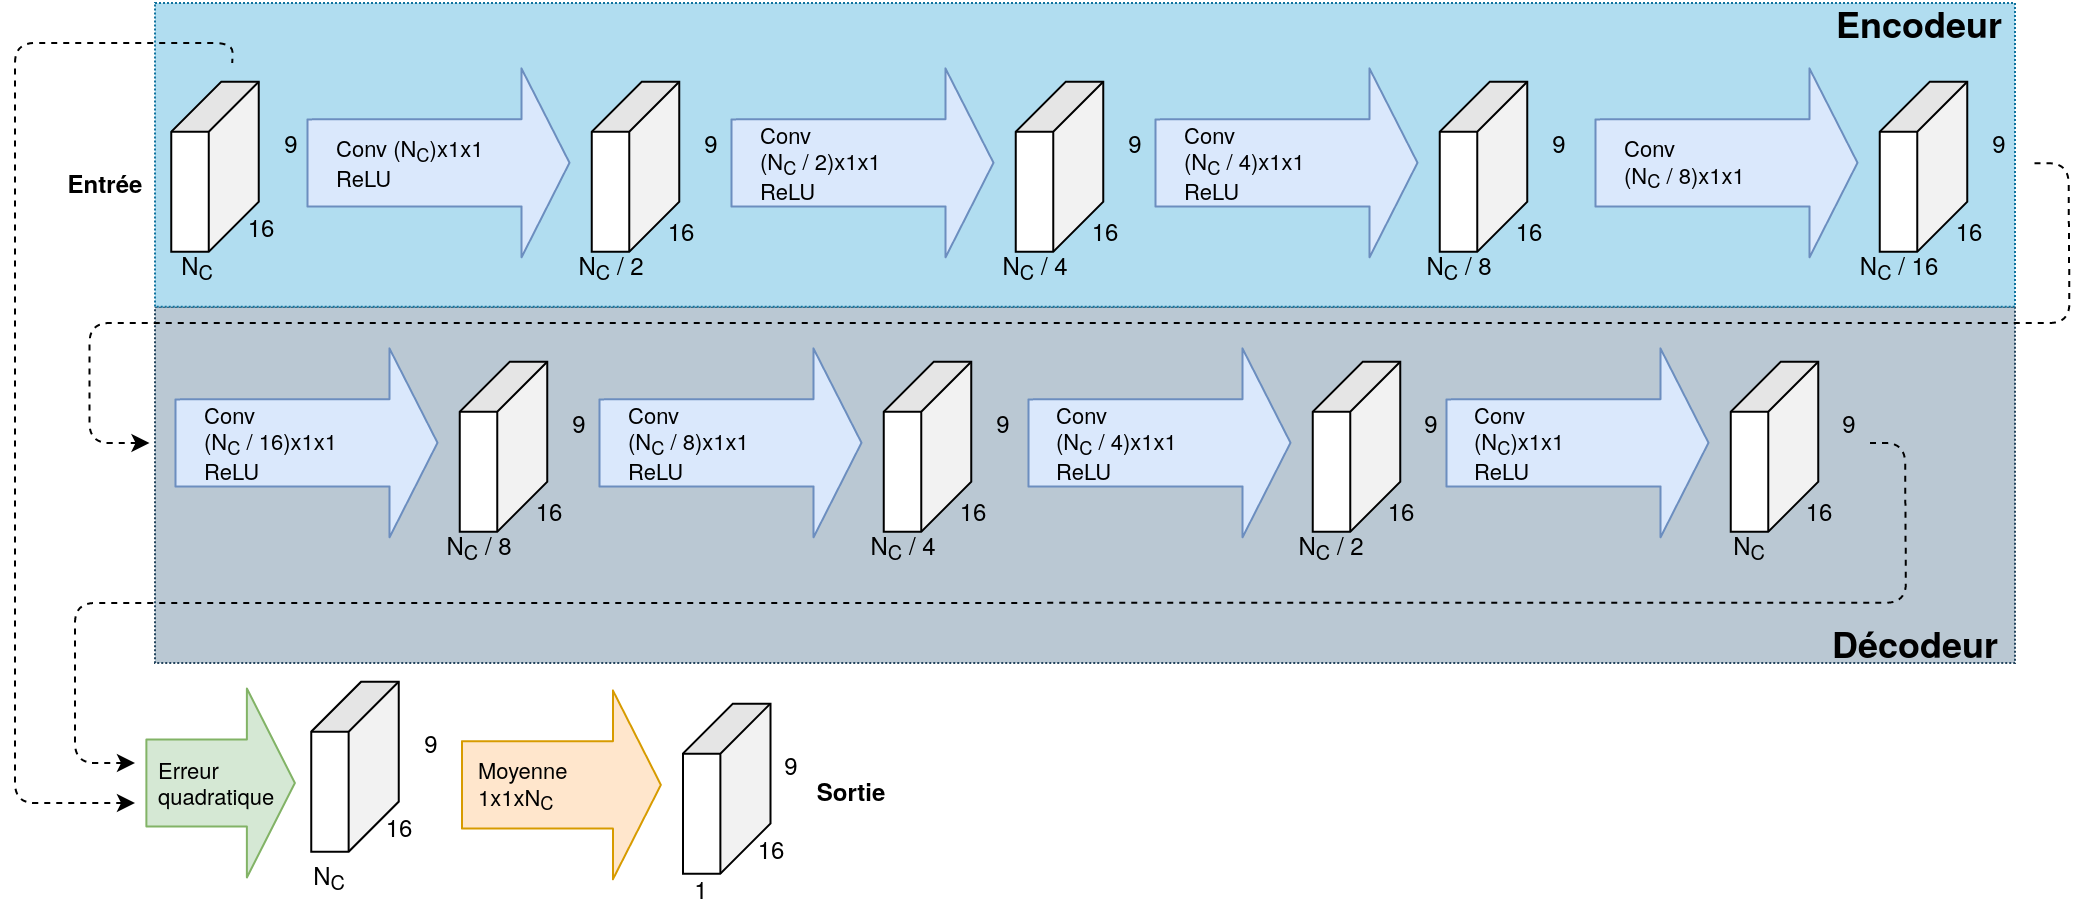
\includegraphics[width=17cm]{images/Architecture_FeatureAutoencoder.png}
        \caption{Architecture de l'auto-encodeur des caractéristiques}
        \label{fig:architecture_autoencoder_caracteristique}
    \end{figure}

\subsubsection{Auto-encodeur à base de couche convolutive appliqué sur l'image}
    Un réseau de neurones de type auto-encodeur reconstruisant l'image en entrée à été conçu. L'architecture de ce réseau est présentée à la figure \ref{fig:architecture_cnn_autoencoder}. Le réseau est configurable à l'aide de \(N_A\) et de \(N_B\). \(N_A\) permet de choisir le nombre de canaux après la première convolution de l'encodeur, tandis que \(N_B\) permet de choisir le taux de grossissement du nombre de canaux après chaque convolution de l'encodeur. Le décodeur est symétrique par rapport à l'encodeur. À la sortie du décodeur, il y a une interpolation bilinéaire, car il n'était pas possible de respecter en même temps le champ récepteur et le fait que l'image en entrée et celle en sortie aient la même taille parce que certains \textit{MaxPool} ne donnent pas une sortie de type \textit{same}. Alors, la solution la plus simple était d'utiliser une interpolation bilinéaire. La dernière fonction d'activation du décodeur est la fonction sigmoïde parce que les valeurs des pixels d'une image sont entre 0 et 1. La sortie du réseau de neurones est l'erreur quadratique moyenne de la reconstruction de chaque région. Ce réseau de neurones sera appelé modèle A dans la suite du document.
    \begin{figure}[H]
        \centering
        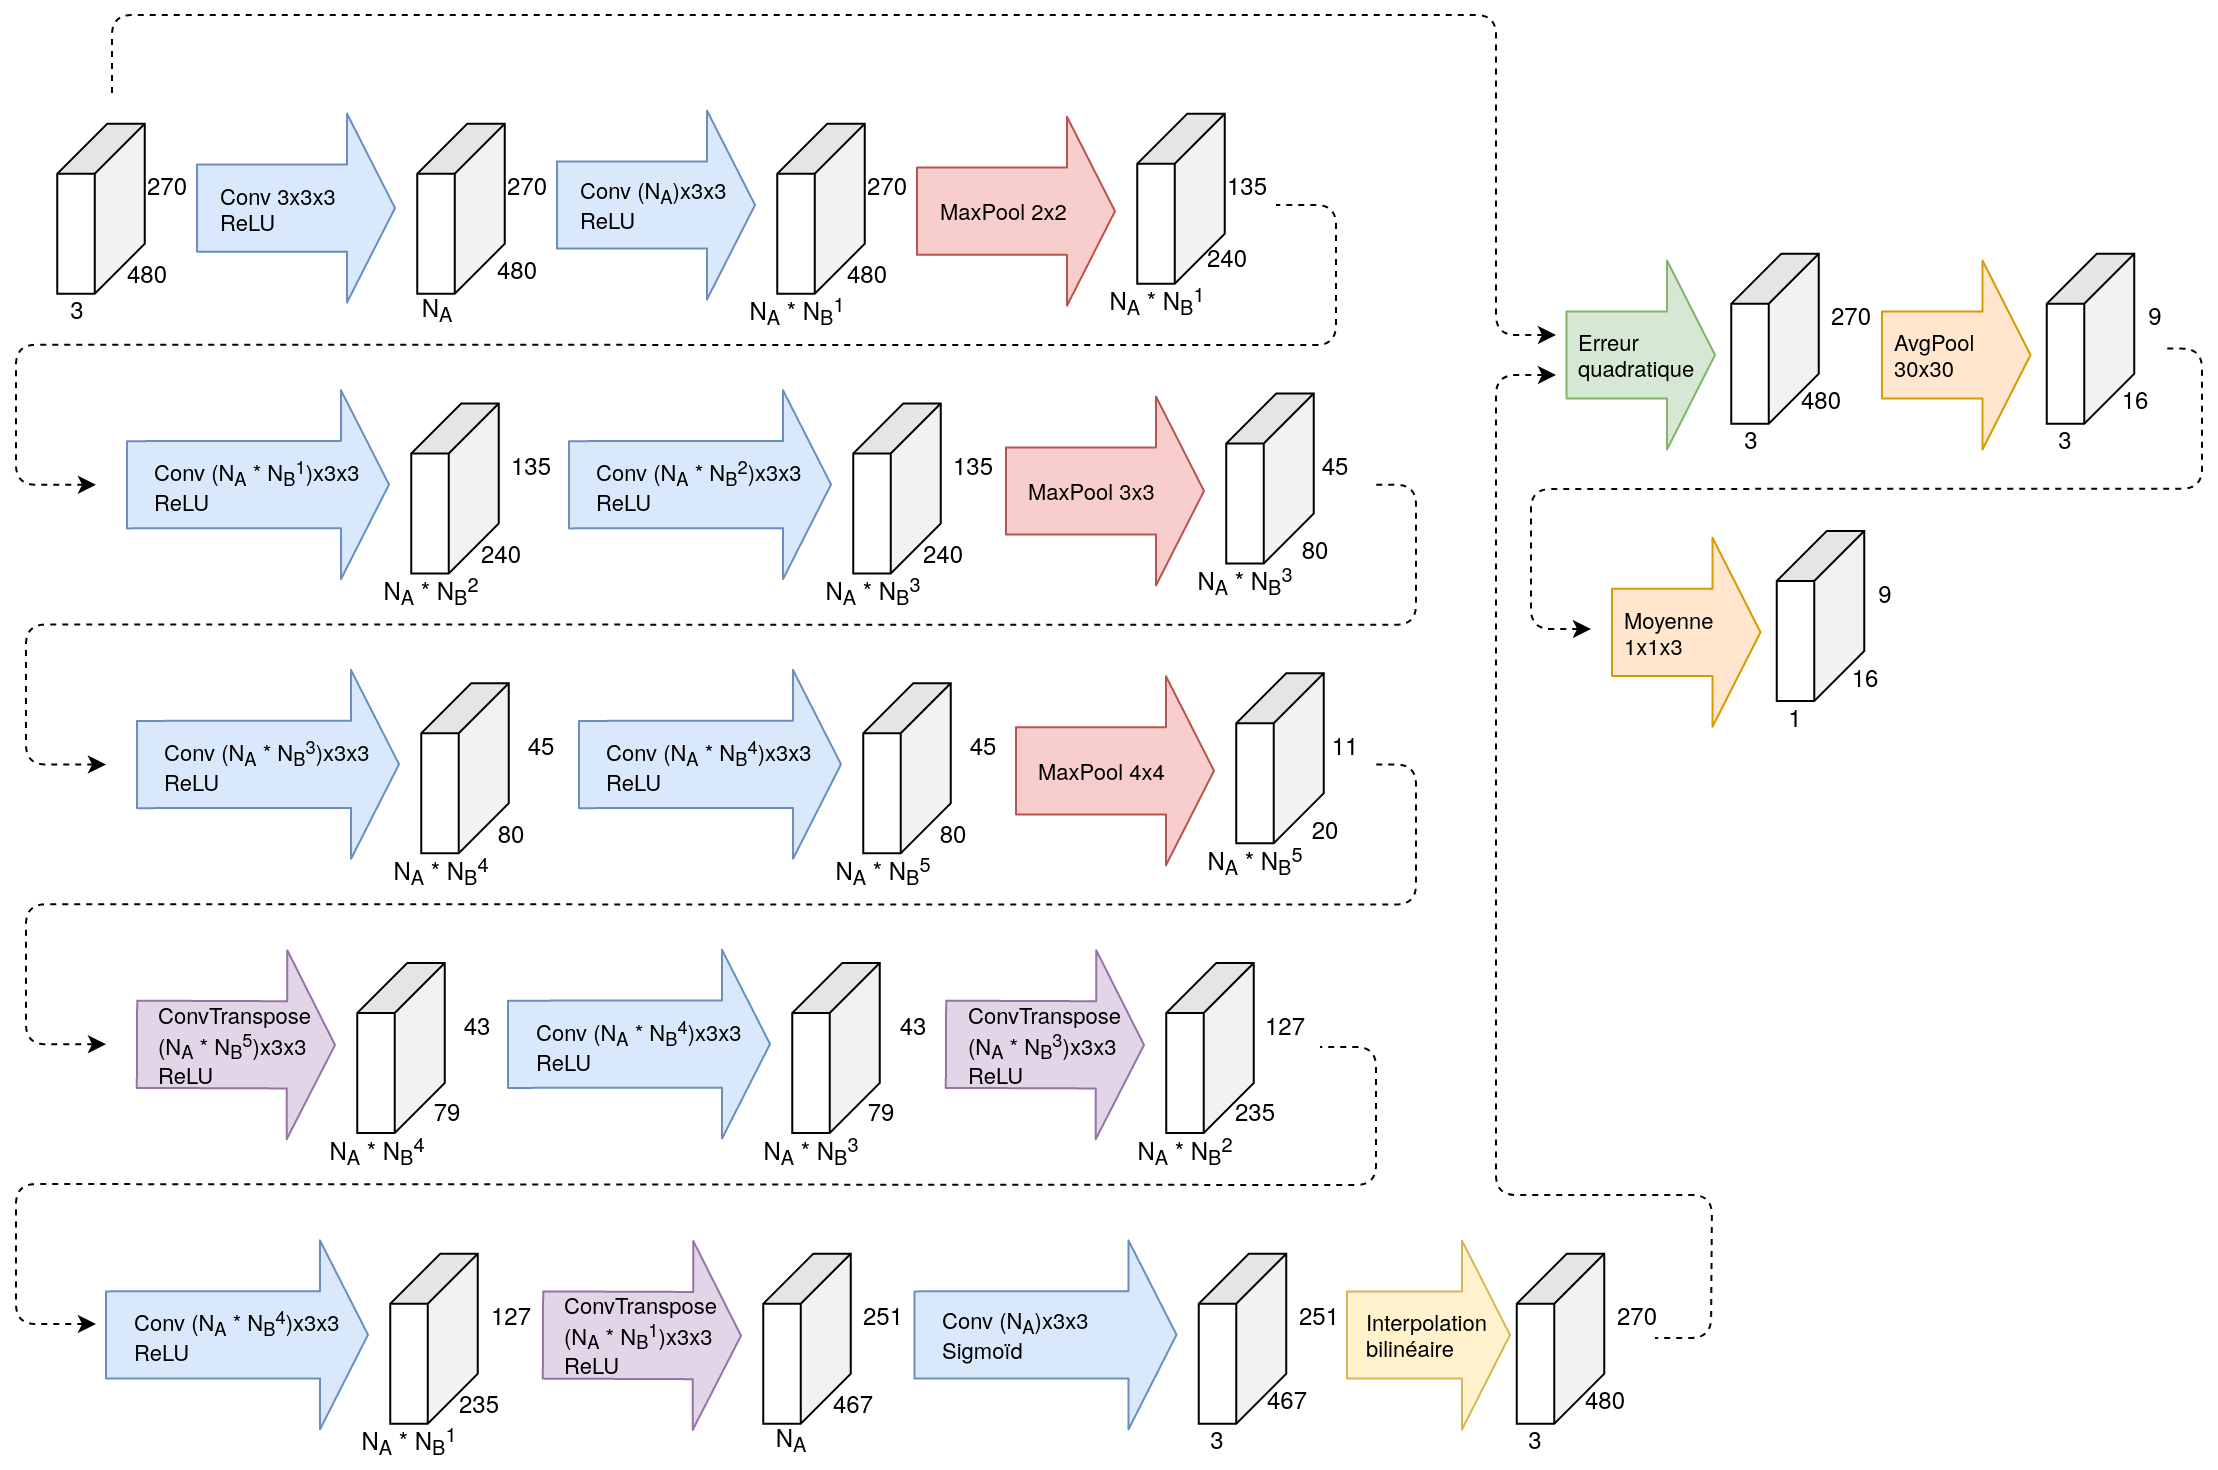
\includegraphics[width=17cm]{images/Architecture_CnnAutoencoder.png}
        \caption{Architecture de l'auto-encodeur à base de couche convolutive appliqué sur l'image}
        \label{fig:architecture_cnn_autoencoder}
    \end{figure}

\subsubsection{Auto-encodeur variationnel à base de couche convolutive appliqué sur l'image}
    Il a été décidé de développer un auto-encodeur variationnel dans le but de vérifier si le fait de contraindre la sortie de l'encodeur permet d'améliorer les performances. Par conséquent, l'architecture de l'auto-encodeur variationnel présenté à la figure \ref{fig:architecture_cnn_vae} est très semblable à celle du modèle A. Les seules différences concernent la sortie de l'encodeur et l'entrée du décodeur. La sortie de l'encodeur correspond à une distribution de probabilité normale multidimensionnelle où la matrice de covariance est une diagonale. L'entrée du décodeur est un point échantillonné la cette distribution de probabilité. Ce réseau de neurones sera appelé modèle B dans la suite du document.
    \begin{figure}[H]
        \centering
        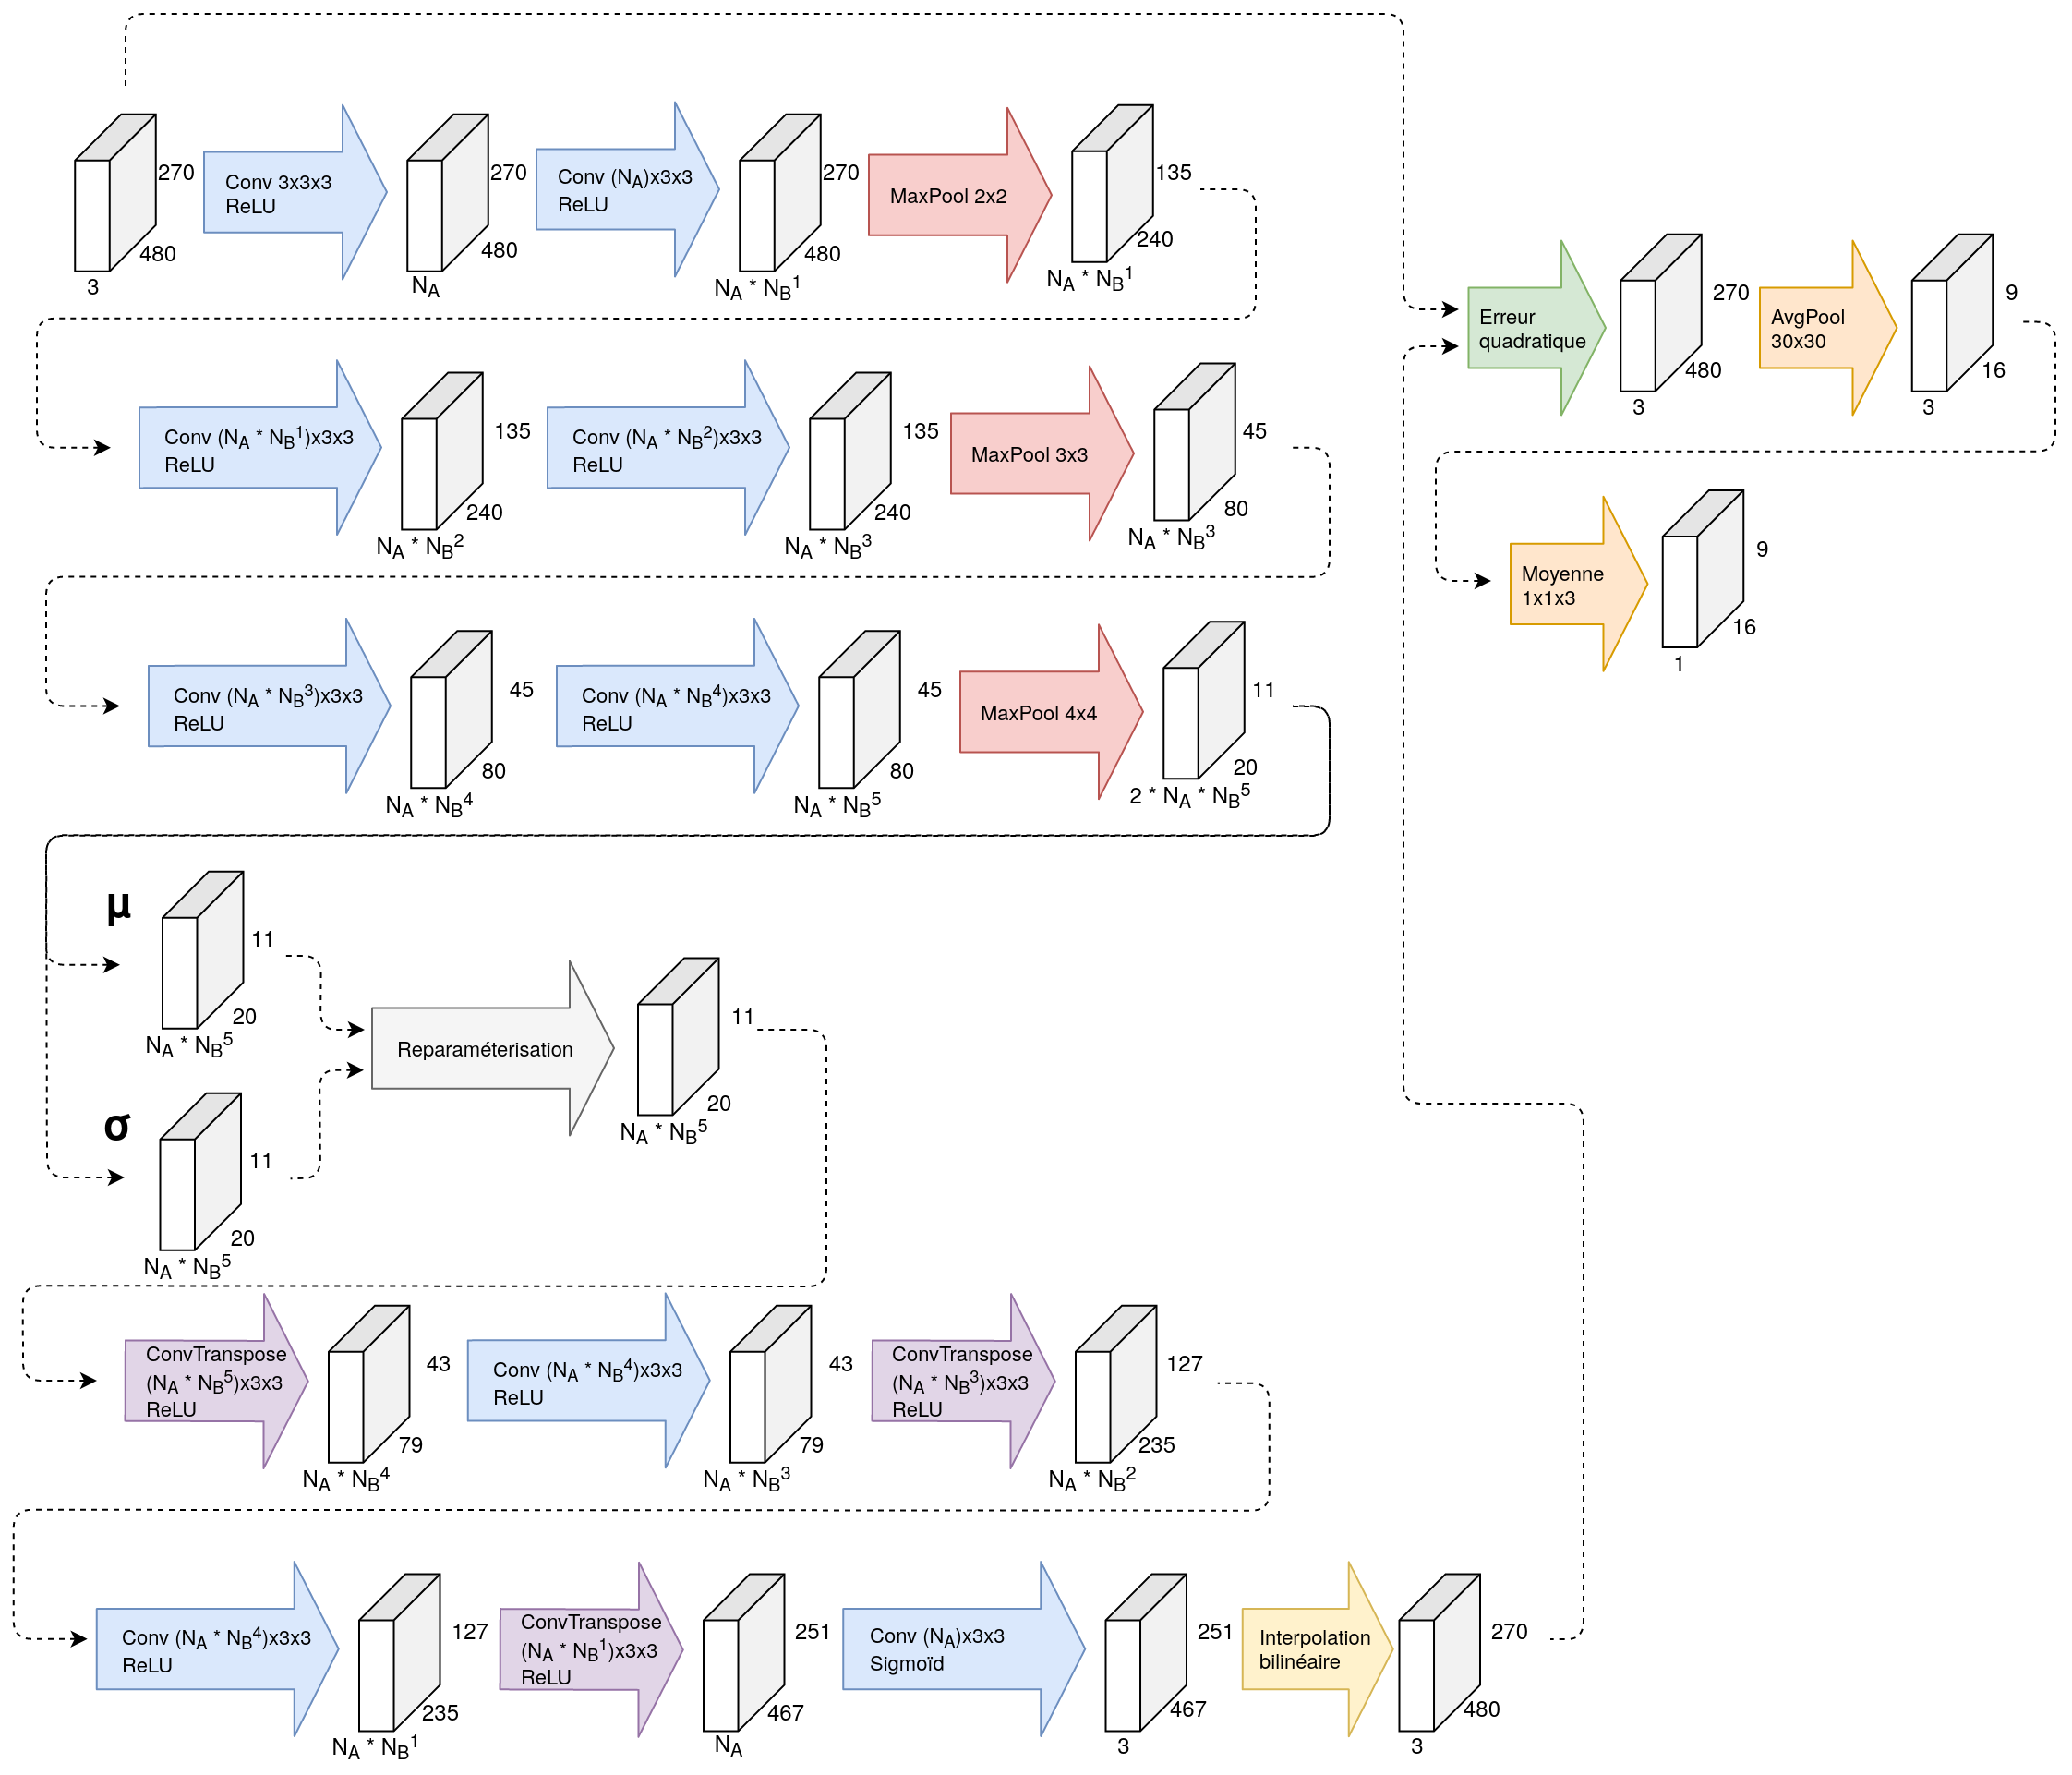
\includegraphics[width=17cm]{images/Architecture_CnnVae.png}
        \caption{Architecture de l'auto-encodeur variationnel à base de couche convolutive appliqué sur l'image}
        \label{fig:architecture_cnn_vae}
    \end{figure}

\subsubsection{Réseau de neurones convolutif extrayant des caractéristiques}
    La sortie du réseau de neurones convolutif présenté à la figure \ref{fig:architecture_small_cnn} est envoyée à l'entrée de l'auto-encodeur des caractéristiques (figure \ref{fig:architecture_autoencoder_caracteristique}) pour que la sortie de l'auto-encodeur des caractéristiques soit les erreurs de reconstruction des régions. Le réseau de neurones convolutif sert extraire des caractéristiques de chaque région de l'image. Le réseau est configurable à l'aide de \(N_A\) et de \(N_B\). Les effets de ces paramètres sont les mêmes que dans le modèle A. À la sortie du réseau de neurones convolutif, il y a l'application d'une \textit{BatchNorm} dans le but de limiter la plage dynamique des caractéristiques de chaque région et d'une interpolation bilinéaire pour obtenir la bonne taille. L'interpolation bilinéaire est nécessaire pour les mêmes raisons que le modèle A. La combinaison de ces deux réseaux de neurones sera appelée modèle C dans la suite du document.
    \begin{figure}[H]
        \centering
        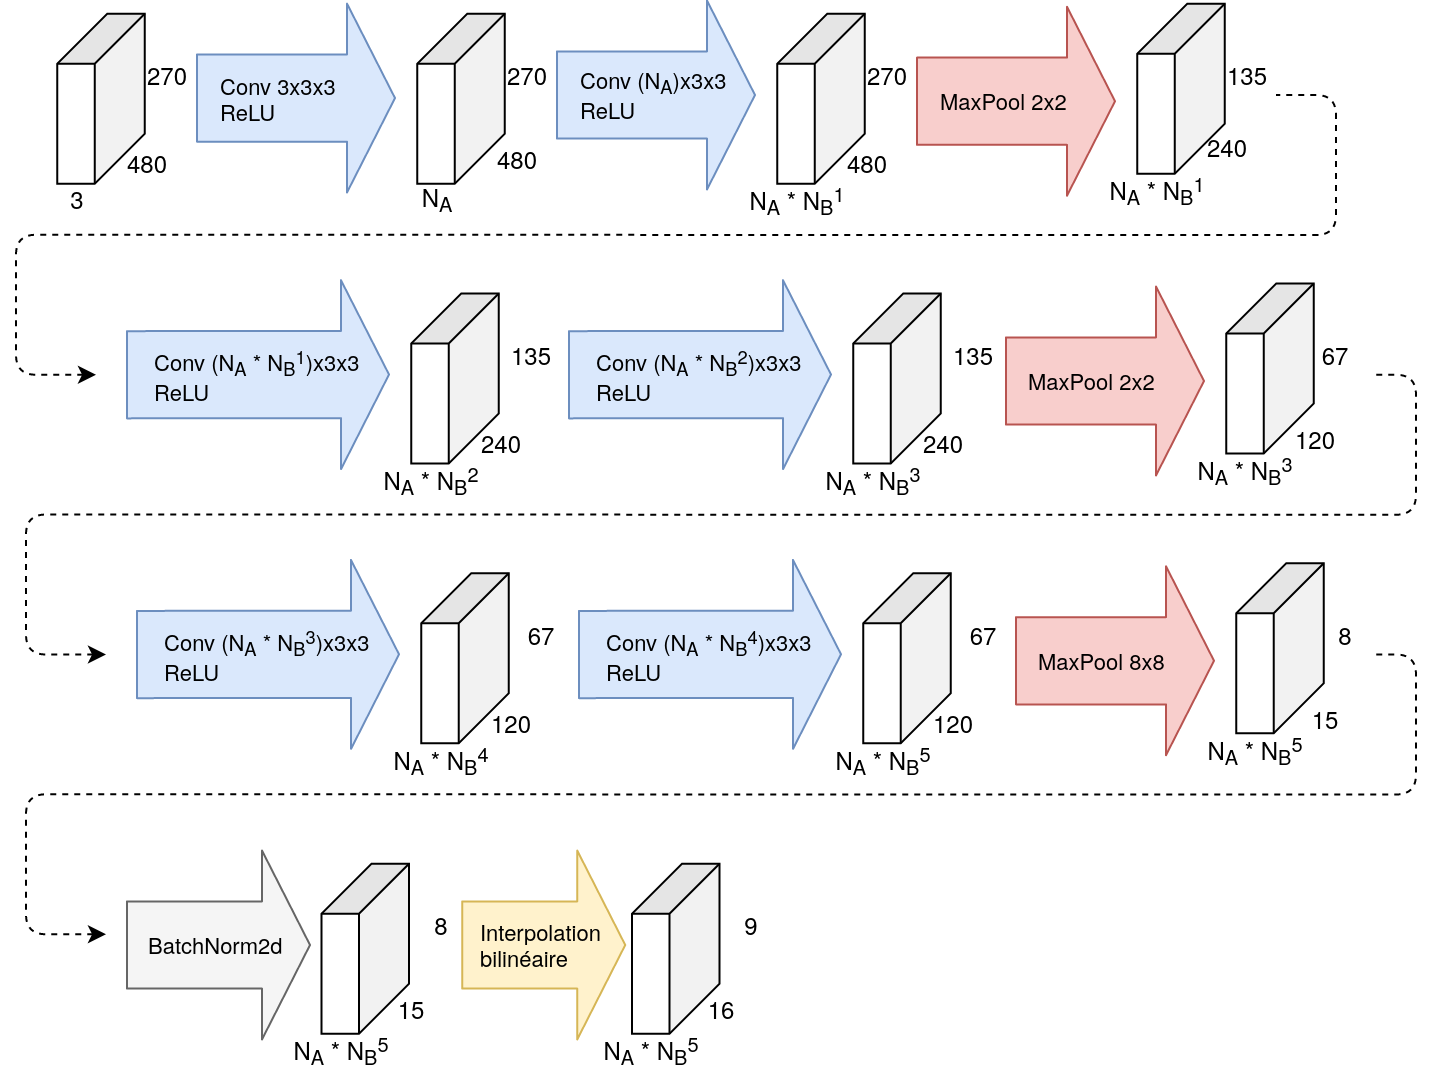
\includegraphics[width=17cm]{images/Architecture_SmallCnnWithAutoencoder.png}
        \caption{Architecture du réseau de neurones convolutif extrayant des caractéristiques}
        \label{fig:architecture_small_cnn}
    \end{figure}

\subsubsection{Réseau de neurones à base de blocs denses extrayant des caractéristiques}
    \begin{figure}[H]
        \centering
        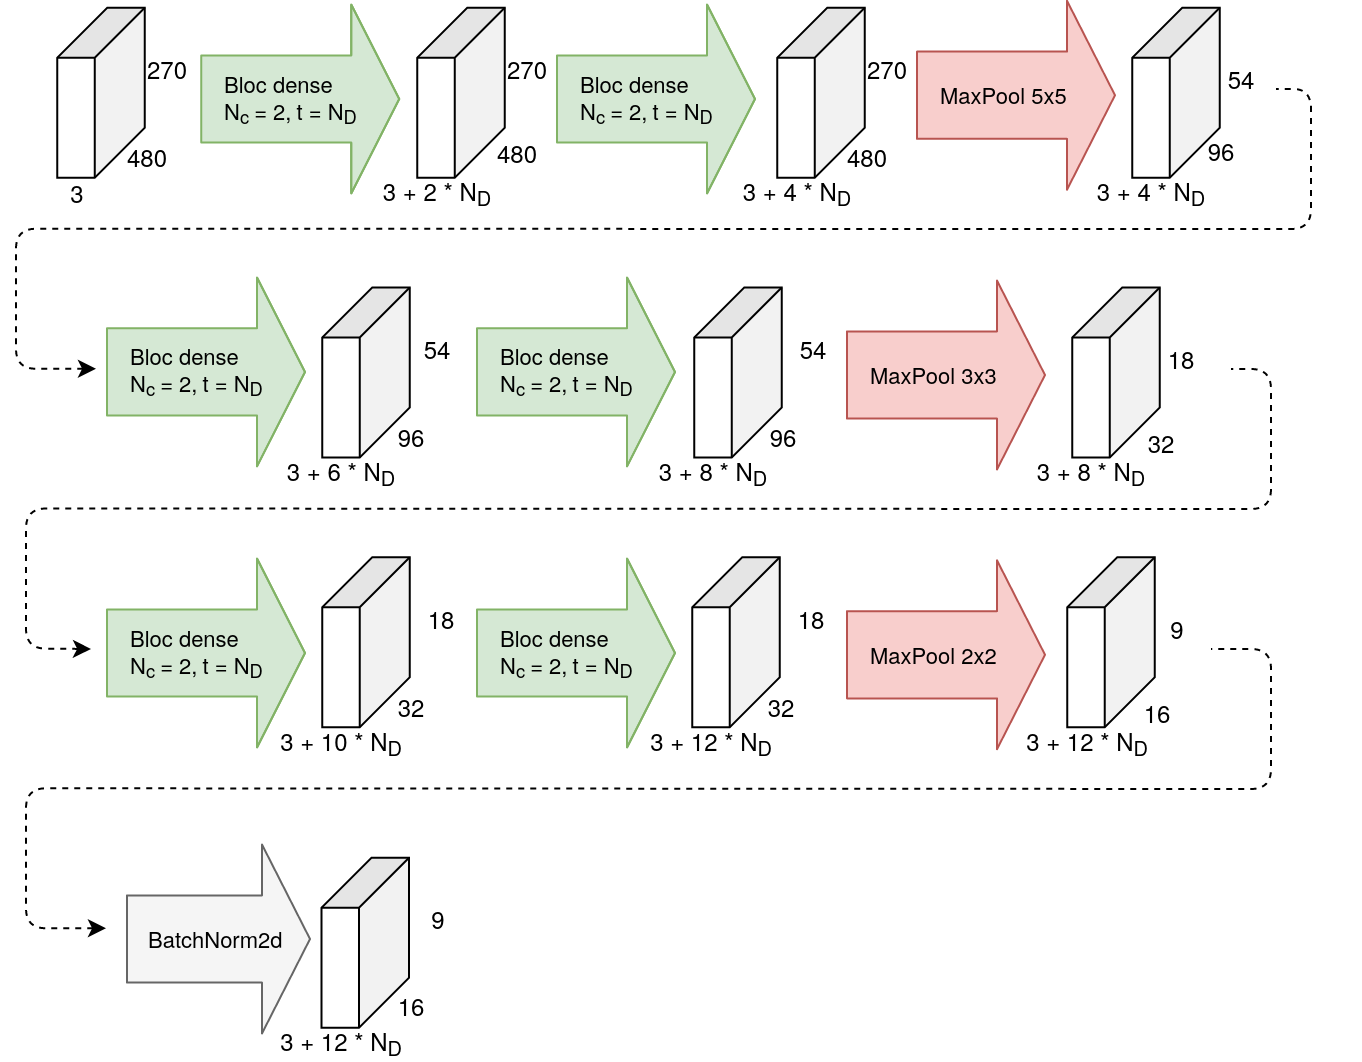
\includegraphics[width=17cm]{images/Architecture_SmallCnnWithAutoencoderDenseBlocks.png}
        \caption{Architecture du réseau de neurones à base de blocs denses extrayant des caractéristiques}
        \label{fig:architecture_small_cnn_dense_bloc}
    \end{figure}

\subsection{Réseau de neurones utilisant un \textit{backend} VGG16 pour l'extraction des caractéristiques}
    La sortie du réseau de neurones utilisant un \textit{backend} VGG16 présenté à la figure \ref{fig:architecture_vgg16} est envoyée à l'entrée de l'auto-encodeur des caractéristiques (figure \ref{fig:architecture_autoencoder_caracteristique}) pour que la sortie de l'auto-encodeur des caractéristiques soit les erreurs de reconstruction des régions. Les 8 premières couches de VGG16, suivi d'un \textit{MaxPool} 8x8 a été utilisé pour obtenir le bon champ récepteur. Il y a l'utilisation d'une \textit{BatchNorm} et d'une interpolation bilinéaire pour les mêmes raisons que le modèle C. La combinaison de ces deux réseaux de neurones sera appelée modèle E dans la suite du document.
    \begin{figure}[H]
        \centering
        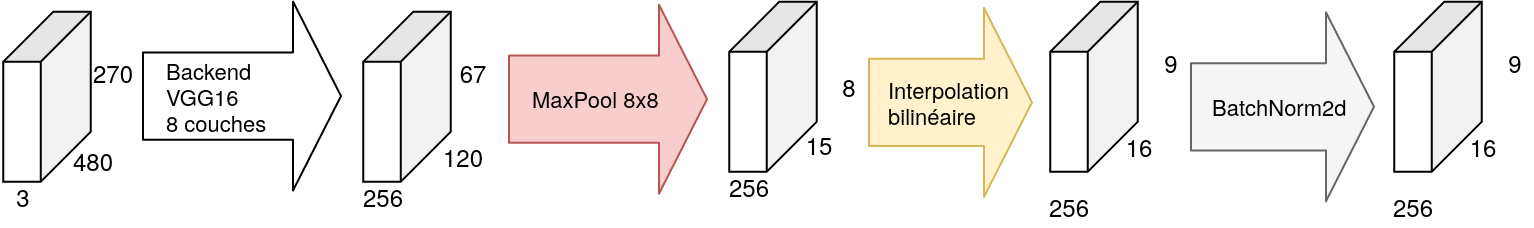
\includegraphics[width=12cm]{images/Architecture_Vgg16BackendAutoencoder.png}
        \caption{Architecture du réseau de neurones utilisant un \textit{backend} VGG16 pour l'extraction des caractéristiques}
        \label{fig:architecture_vgg16}
    \end{figure}

\subsection{Augmentation des données}
    
    \section{Entraînement}
    Il a été décidé de faire l'entraînement des réseaux de neurones sur 10 époques, car l'entraînement doit être rapide dans ce contexte.
    
\section{Résultats}

\subsection{Courbes d'apprentissage}

    \begin{figure}[H]
        \centering
        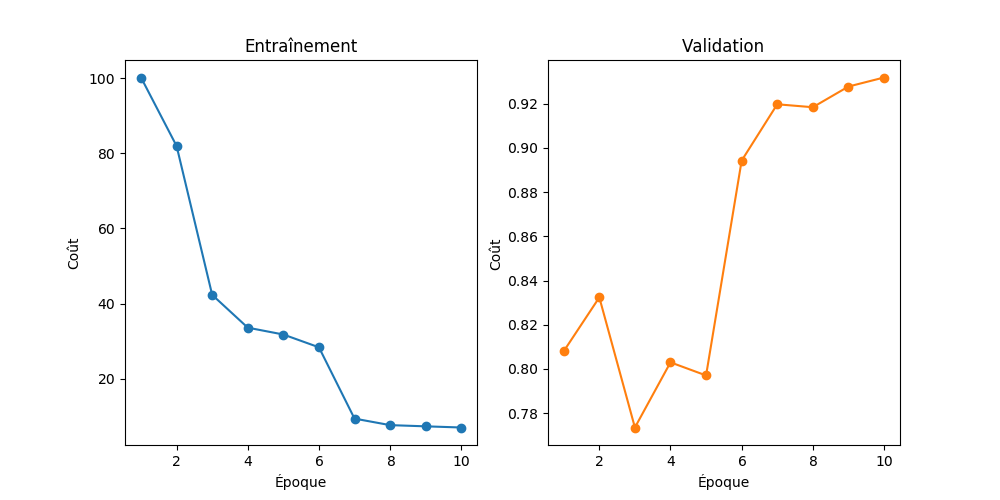
\includegraphics[width=16cm]{images/learning_curves_a.png}
        \caption{Exemple de courbe d'apprentissage du modèle A}
        \label{fig:learning_curves_a}
    \end{figure}

    \begin{figure}[H]
        \centering
        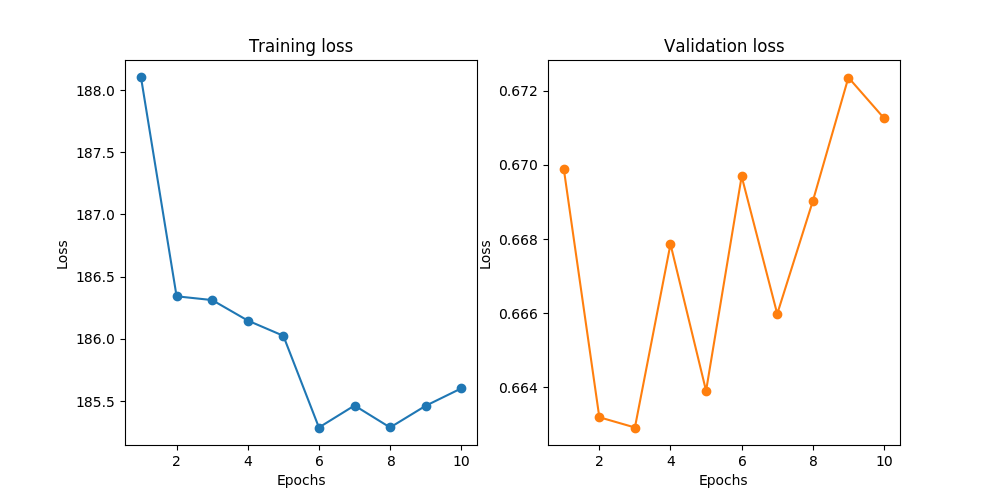
\includegraphics[width=16cm]{images/learning_curves_b.png}
        \caption{Exemple de courbe d'apprentissage du modèle B}
        \label{fig:learning_curves_b}
    \end{figure}

    \begin{figure}[H]
        \centering
        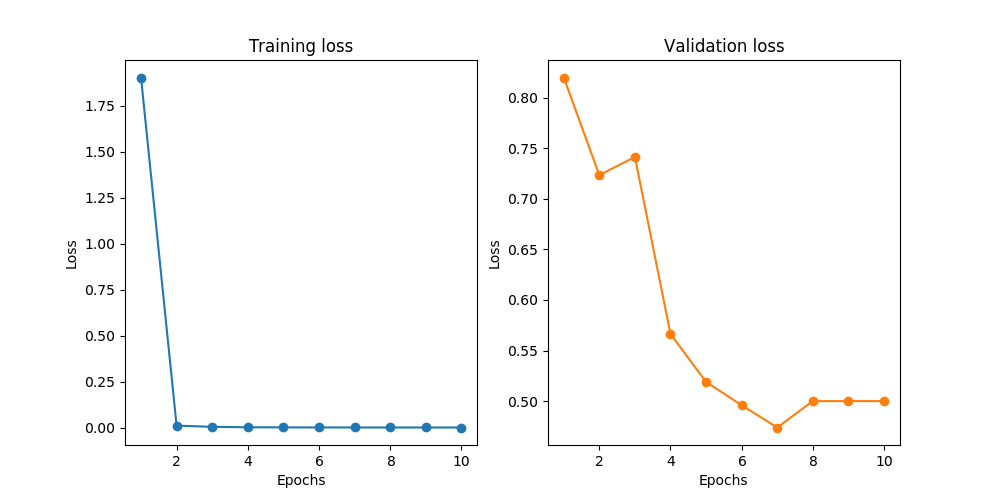
\includegraphics[width=16cm]{images/learning_curves_c.png}
        \caption{Exemple de courbe d'apprentissage du modèle C}
        \label{fig:learning_curves_c}
    \end{figure}

    \begin{figure}[H]
        \centering
        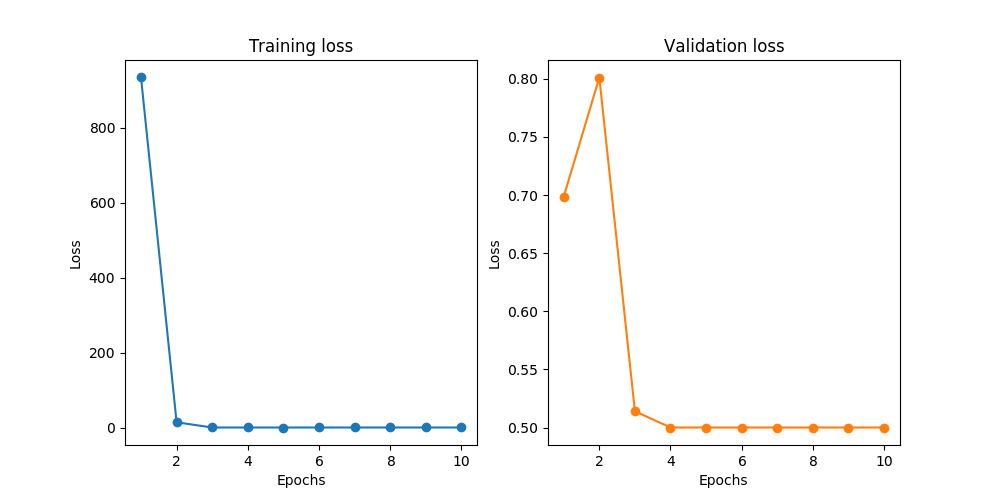
\includegraphics[width=16cm]{images/learning_curves_d.png}
        \caption{Exemple de courbe d'apprentissage du modèle D}
        \label{fig:learning_curves_d}
    \end{figure}

\subsection{Base de données - Tunnel}

\subsubsection{Recherche des hyperparamètres}
    \begin{table}[H]
        \centering
        \caption{Résultat de la recherche des hyperparamètres du modèle A - Tunnel}
        \label{tab:resultat_tunnel_modele_a}
        \begin{tabular}{lllp{3cm}p{3cm}l}
            \midrule
            \# & \(N_A\) & \(N_B\) & Augmentation des données & Métrique de validation & Époque\\
            \midrule\midrule
            1  & 2 & 2 & Non & 0,812 & 10\\
            2  & 2 & 2 & Oui & \\
            3  & 2 & 3 & Non & 0,614 & 1\\
            4  & 2 & 3 & Oui & 0,791 & 7\\
            5  & 4 & 2 & Non & 0,933 & 7\\
            6  & 4 & 2 & Oui & 0,932 & 10\\
            7  & 4 & 3 & Non & 0,930 & 7\\
            \textbf{8}  & \textbf{4} & \textbf{3} & \textbf{Oui} & \textbf{0,936} & \textbf{10}\\
            9  & 8 & 2 & Non & 0,934 & 4\\
            10 & 8 & 2 & Oui & 0,935 & 10\\
            \midrule
        \end{tabular}
    \end{table}

    \begin{table}[H]
        \centering
        \caption{Résultat de la recherche des hyperparamètres du modèle B - Tunnel}
        \label{tab:resultat_tunnel_modele_b}
        \begin{tabular}{lllp{3cm}p{3cm}l}
            \midrule
            \# & \(N_A\) & \(N_B\) & Augmentation des données & Métrique de validation & Époque\\
            \midrule\midrule
            1  & 2 & 2 & Non & 0,612 & 9\\
            2  & 2 & 2 & Oui & 0,673 & 10\\
            3  & 2 & 3 & Non & 0,634 & 1\\
            4  & 2 & 3 & Oui & 0,673 & 6\\
            5  & 4 & 2 & Non & 0,613 & 6\\
            \textbf{6}  & \textbf{4} & \textbf{2} & \textbf{Oui} & \textbf{0,673} & \textbf{2}\\
            7  & 4 & 3 & Non & 0,621 & 4\\
            8  & 4 & 3 & Oui & 0,672 & 9\\
            9  & 8 & 2 & Non & 0,632 & 2\\
            10 & 8 & 2 & Oui & 0,672 & 6\\
            \midrule
        \end{tabular}
    \end{table}

    \begin{table}[H]
        \centering
        \caption{Résultat de la recherche des hyperparamètres du modèle E - Tunnel}
        \label{tab:resultat_tunnel_modele_e}
        \begin{tabular}{lp{3cm}p{3cm}p{3cm}l}
            \midrule
            \# & Entraînement du \text{backend} & Augmentation des données & Métrique de validation & Époque\\
            \midrule\midrule
            \textbf{1} & \textbf{Non} & \textbf{Non} & \textbf{0,931} & \textbf{10}\\
            2 & Non & Oui & 0,926 & 9\\
            3 & Oui & Non & 0,500 & 8\\
            4 & Oui & Oui & 0,500 & 8\\
            \midrule
        \end{tabular}
    \end{table}

\subsubsection{Comparaison entre les modèles}
    \begin{figure}[H]
        \centering
        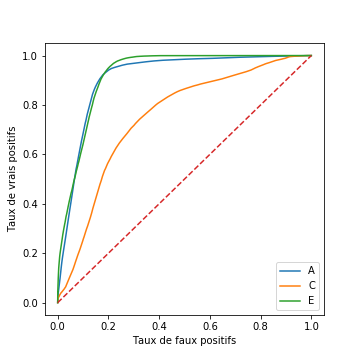
\includegraphics[width=8cm]{images/tunnel_roc.png}
        \caption{Courbes ROC - Tunnel}
        \label{fig:tunnel_roc}
    \end{figure}

    \begin{table}[H]
        \centering
        \caption{Temps d'exécution moyen sur Tesla K20 - Tunnel}
        \label{tab:resultat_tunnel_temps_execution}
        \begin{tabular}{lp{4cm}p{4cm}p{4cm}}
            \midrule
            Modèle & Temps d'exécution moyen de la passe avant (ms) & Temps d'exécution moyen de la passe arrière (ms) & Temps d'exécution total moyen (ms)\\
            \midrule\midrule
            A & 2,93 & 4,75 & 7,68\\
            B & 3,65 & 5,86 & 9,51\\
            E & 3,14 & 2,78 & 5,92\\
            \midrule
        \end{tabular}
    \end{table}

\subsection{Base de données - Faculté de génie}

\subsubsection{Recherche des hyperparamètres}
    \begin{table}[H]
        \centering
        \caption{Résultat de la recherche des hyperparamètres du modèle A - Faculté de génie}
        \label{tab:resultat_corridor_modele_a}
        \begin{tabular}{lllp{3cm}p{3cm}l}
            \midrule
            \# & \(N_A\) & \(N_B\) & Augmentation des données & Métrique de validation & Époque\\
            \midrule\midrule
            1  & 2 & 2 & Non & 0,501 & 1\\
            2  & 2 & 2 & Oui & 0,610 & 7\\
            3  & 2 & 3 & Non & 0,665 & 8\\
            4  & 2 & 3 & Oui & 0,644 & 10\\
            \textbf{5}  & \textbf{4} & \textbf{2} & \textbf{Non} & \textbf{0,678} & \textbf{10}\\
            6  & 4 & 2 & Oui & 0,652 & 10\\
            7  & 4 & 3 & Non & 0,677 & 10\\
            8  & 4 & 3 & Oui & 0,666 & 7\\
            9  & 8 & 2 & Non & 0,667 & 9\\
            10 & 8 & 2 & Oui & 0,672 & 10\\
            \midrule
        \end{tabular}
    \end{table}
    
    \begin{table}[H]
        \centering
        \caption{Résultat de la recherche des hyperparamètres du modèle B - Faculté de génie}
        \label{tab:resultat_corridor_modele_b}
        \begin{tabular}{lllp{3cm}p{3cm}l}
            \midrule
            \# & \(N_A\) & \(N_B\) & Augmentation des données & Métrique de validation & Époque\\
            \midrule\midrule
            1  & 2 & 2 & Non & 0,499 & 7\\
            2  & 2 & 2 & Oui & 0,503 & 5\\
            3  & 2 & 3 & Non & 0,499 & 10\\
            4  & 2 & 3 & Oui & 0,502 & 4\\
            \textbf{5}  & \textbf{4} & \textbf{2} & \textbf{Non} & \textbf{0,511} & \textbf{1}\\
            6  & 4 & 2 & Oui & 0,501 & 10\\
            7  & 4 & 3 & Non & 0,501 & 8\\
            8  & 4 & 3 & Oui & 0,500 & 2\\
            9  & 8 & 2 & Non & 0,499 & 1\\
            10 & 8 & 2 & Oui & 0,501 & 10\\
            \midrule
        \end{tabular}
    \end{table}
    
    \begin{table}[H]
        \centering
        \caption{Résultat de la recherche des hyperparamètres du modèle E - Faculté de génie}
        \label{tab:resultat_corridor_modele_e}
        \begin{tabular}{lp{3cm}p{3cm}p{3cm}l}
            \midrule
            \# & Entraînement du \text{backend} & Augmentation des données & Métrique de validation & Époque\\
            \midrule\midrule
            \textbf{1} & \textbf{Non} & \textbf{Non} & \textbf{0,719} & \textbf{10}\\
            2 & Non & Oui & 0,699 & 7\\
            3 & Oui & Non & 0,500 & 10\\
            4 & Oui & Oui & 0,500 & 10\\
            \midrule
        \end{tabular}
    \end{table}

\subsubsection{Comparaison entre les modèles}
    \begin{figure}[H]
        \centering
        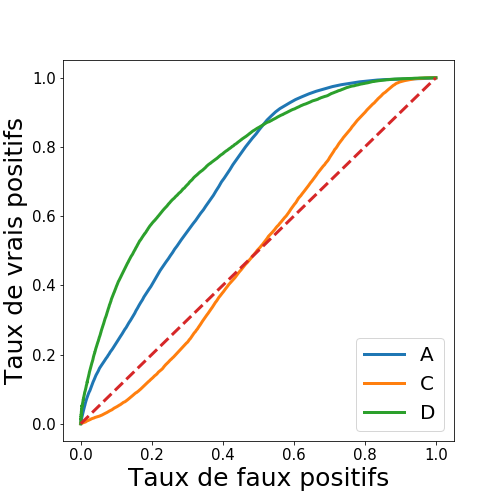
\includegraphics[width=8cm]{images/corridor_roc.png}
        \caption{Courbes ROC - Faculté de génie}
        \label{fig:corridor_roc}
    \end{figure}

    \begin{table}[H]
        \centering
        \caption{Temps d'exécution moyen sur Tesla K20 - Faculté de génie}
        \label{tab:resultat_corridor_temps_execution}
        \begin{tabular}{lp{4cm}p{4cm}p{4cm}}
            \midrule
            Modèle & Temps d'exécution moyen de la passe avant (ms) & Temps d'exécution moyen de la passe arrière (ms) & Temps d'exécution total moyen (ms)\\
            \midrule\midrule
            A & 3,08 & 4,22 & 7,30\\
            B & 3,65 & 5,86 & 9,51\\
            E & 3,14 & 2,78 & 5,92\\
            \midrule
        \end{tabular}
    \end{table}

\subsection{Analyse générale}
    
    \section{Gestion de projet}
    L'outil de contrôle de versions retenu pour le projet est un Git hébergé par Microsoft (\url{https://github.com/mamaheux/CuriousNetwork}). Les tableaux de type Trello de GitHub ont également été utilisés pour gérer l'assignation et le suivi des tâches de développement. Un tableau a été créé pour chaque volet majeur du projet. Une vue d'ensemble des tableaux est présenté à la figure \ref{fig:trello_boards}.

    \begin{figure}[H]
        \centering
        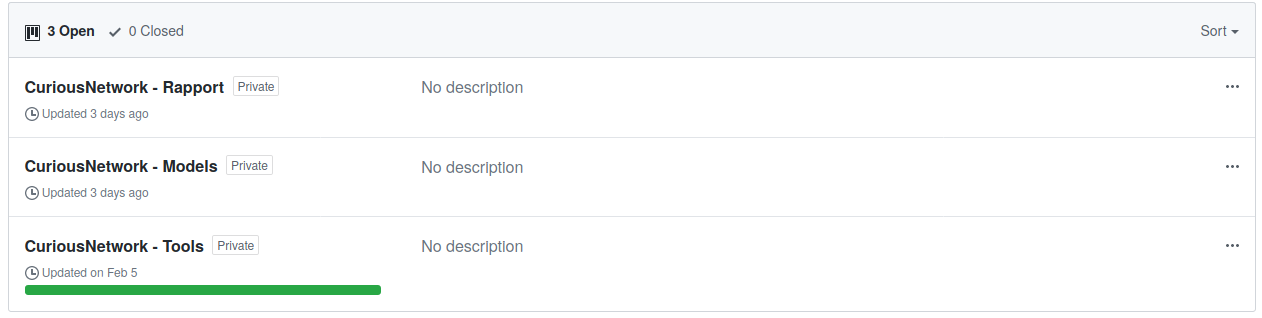
\includegraphics[width=15cm]{images/3_sub_projects.png}
        \caption{Tableaux de suivi des tâches de chaque volet du projet}
        \label{fig:trello_boards}
    \end{figure}

    La figure \ref{fig:trello_board_models} présente un aperçu du tableau de suivi pour le volet des modèles de réseaux de neurones.
    \begin{figure}[H]
        \centering
        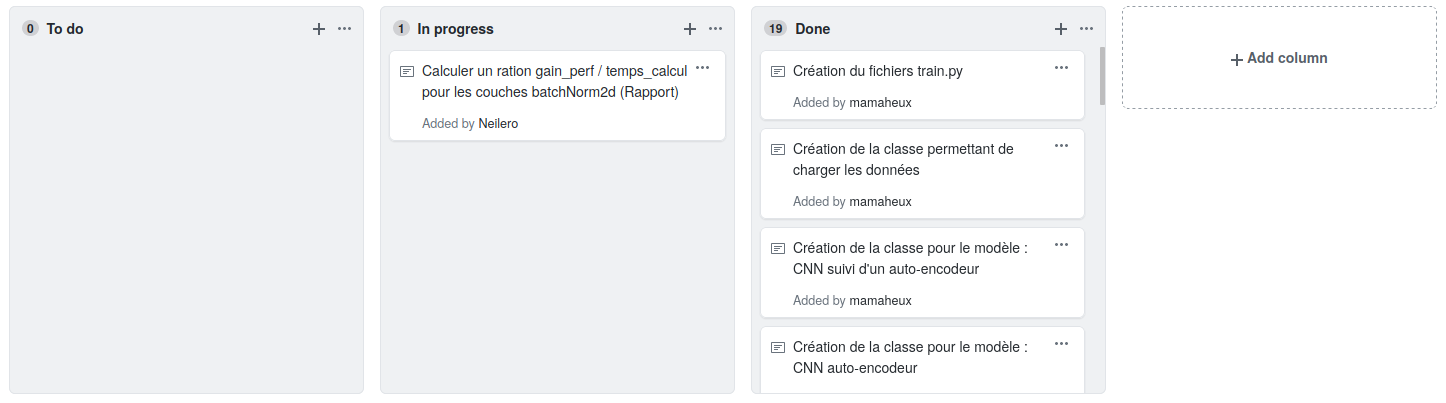
\includegraphics[width=15cm]{images/trello_board.png}
        \caption[Tableau Trello du volet modèles]{Tableau Trello du volet \textbf{modèles}}
        \label{fig:trello_board_models}
    \end{figure}

    Pour suivre les bonnes pratiques, chaque tâche de développement a été effectuée sur sa propre branche. Une fois la tâche complétée, la branche faisait l'objet d'une demande \textit{pull request} et devait être révisée par un autre membre de l'équipe avant de pouvoir être fusionnée (\textit{merge}) à la branche principale \textit{master}. Une fois les branches fusionnées, elles étaient supprimées.\\
    
    Les \textit{commits} ont été effectués de manière à avoir la plus grande granularité possible de manière à simplifier les révisions de codes ainsi que la traçabilité. Il a été décidé de ne pas utiliser de \textit{squash and merge} afin de conserver l'historique de l'évolution du code pour chaque fusion. La figure \ref{fig:git_graph} présente un aperçu de l'arborescence Git du projet.
    \begin{figure}[H]
        \centering
        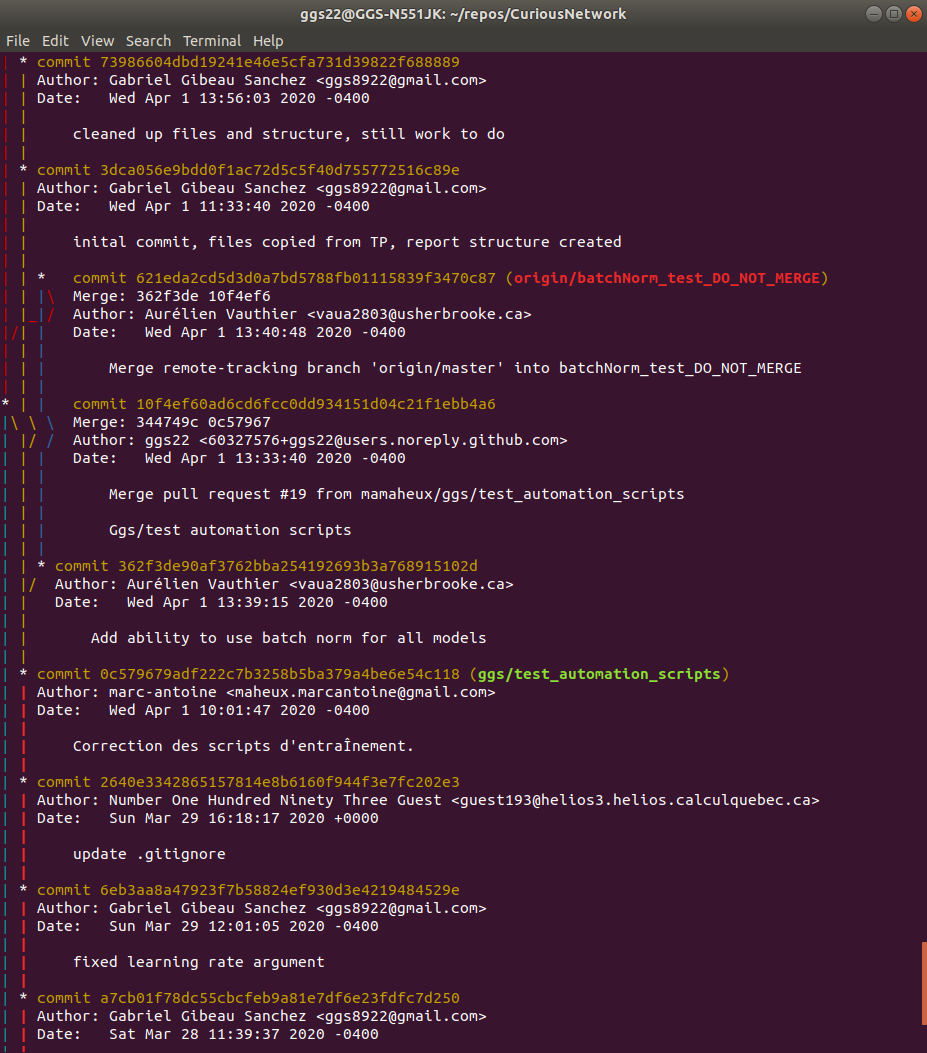
\includegraphics[width=15cm]{images/git_graph.png}
        \caption{Apperçu de l'arborescence du Git}
        \label{fig:git_graph}
    \end{figure}
    \section{Conclusion et pistes de recherche futures}
    Toutes les expérimentations ont permis de valider l'utilisation d'un auto-encodeur dans un système d'attention si certaines contraintes sont respectées. De plus, il a été possible de déterminer les problèmes de différents modèles, de déterminer le meilleur modèle et d'invalider un modèle. Pour compléter l'étude actuelle, il serait intéressant de réaliser les éléments suivants.

    \begin{itemize}
        \item Tester avec d'autres \textit{backend} pour l'extraction des caractéristiques dans le but d'améliorer les performances;
        \item Ajouter un terme à la fonction de coût d'entraînement sur le tenseur des caractéristiques des modèles C et D  pour permet l'entraînement du réseau d'extraction des caractéristiques dans le but d'éviter la détérioration des performances de validation au fil de l'entraînement;
        \item Tester les modèles sur d'autres bases de données pour s'assurer de la validité de nos conclusions dans d'autres environnements;
        \item Prendre en compte l'aspect temporel des images des vidéos;
        \item Faire des tests supplémentaires pour mesurer l'effet de l'augmentation des données de contexte
        \item Tester avec un robot possédant un mécanisme d'attention comme celui de HBBA;
        \item Rendre la méthode d'annotation plus systématique pour l'établissement du critère de performance.
    \end{itemize}
    
    Ces éléments pourraient permettre d'améliorer les performances des modèles et de généraliser les conclusions de cette étude.
    
    \pagebreak
    \section{Listes des références}
    [1]     Ferland, F., Létourneau, D., Aumont, A., Frémy, J, Legault, M.-A., Lauria, M., Michaud,         F. (2012), "Natural interaction design of a humanoid robot," Journal of Human-Robot         Interaction, 1 (2), 118-134.\\
    
    [2]    Michaud, F., Ferland, F., Létourneau, D., Legault, M.-A., Lauria, M. (2010), “Toward         autonomous, compliant, omnidirectional humanoid robots for natural interaction in real         life settings,” Paladyn Behavioral Robotic Journal, 1(1): 57-65.\\
    
    [3]    Michaud, F., Côté, C., Létourneau, D., Brosseau, Y., Valin, J.-M., Beaudry, É.,             Raïevsky, C., Ponchon, Moisan, P., Lepage, P., Morin, Y., Gagnon, F., Giguère, P.,             Roux, M.-A., Caron, S., Frenette, P., Kabanza, F. (2007), “Spartacus attending the             2005 AAAI Conference,” to be published in Autonomous Robots, Special Issue on the         AAAI Mobile Robot Competitions and Exhibition.\\
    
    [4]    D. Pathak, P. Agrawal, A. A. Efros, et T. Darrell, “Curiosity-driven Exploration by             Self-supervised Prediction,” arXiv:1705.05363, mai 2017.\\\\
    
    % Appendices
    %\renewcommand{\appendixname}{Annexe}
    %\begin{appendices}
    %    \input{annexea}
        
    %\end{appendices}
    \pagebreak
    
    % Bibliography
    \singlespacing
    \renewcommand{\refname}{Bibliographie}
    \bibliographystyle{IEEEtranN}
    %\bibliography{biblio}
    
\end{document}